%%%%%%%%%%%%%%%%%%%%%%%%%%%%%%%%%%%%%%%%%%%%%%%%%%%%%%%%%%%%%%%%%%%%%%
% 
% 	Template for Producing ASP-DAC 2017 Proceedings
% 
%%%%%%%%%%%%%%%%%%%%%%%%%%%%%%%%%%%%%%%%%%%%%%%%%%%%%%%%%%%%%%%%%%%%%%
% History
% ??/??/?? Designed by Hiroaki Kunieda (ASP-DAC '97 Publication Chair)
% 09/22/97 Modified and small bug fixed by Masaharu Imai 
% 	   (ASP-DAC '98 Publication Chair)
% 11/02/98 Modified by Tsuyoshi Isshiki
% 	   (ASP-DAC 2000 TPS Secretary)
% 7/24/00 Modified by Kiyoharu Hamaguchi
% 	   (ASP-DAC 2001 Publication chair)
% 6/18/02 Modified by Kazutoshi Kobayashi
% 	   (ASP-DAC 2003 Publication Co-Chair)
% 5/27/03 Modified by Kiyoharu Hamaguchi
% 	   (ASP-DAC 2004 TPC secretary)
% 6/10/03 Modified by Kazutoshi Kobayashi for Latex2e
% 	   (ASP-DAC 2004 Publication Co-Chair)
% 6/01/05 Modified by Nozomu Togawa
% 	   (ASP-DAC 2006 Publication Chair)
% 6/01/06 Modified by Hiroyuki Ochi
% 	   (ASP-DAC 2007 Publication Chair)
% 5/30/08 Modified by Nozomu Togawa
% 	   (ASP-DAC 2009 Publication Co-Chair)
% 4/30/10 Modified by Masashi Imai
% 	   (ASP-DAC 2011 Publication Chair)
% 3/20/12 Modified by Masashi Imai
% 	   (ASP-DAC 2013 Publication Chair)
% 5/01/14 Modified by Masashi Imai
% 	   (ASP-DAC 2015 Publication Chair)
% 4/24/16 Modified by Masashi Imai
% 	   (ASP-DAC 2017 Publication Chair)
%%%%%%%%%%%%%%%%%%%%%%%%%%%%%%%%%%%%%%%%%%%%%%%%%%%%%%%%%%%%%%%%%%%%%%
% If you have any problem, please contact ASP-DAC 2017 Publication
% Co-Chairs by E-mail at ``aspdac17publication@hal.eit.hirosaki-u.ac.jp.''
%%%%%%%%%%%%%%%%%%%%%%%%%%%%%%%%%%%%%%%%%%%%%%%%%%%%%%%%%%%%%%%%%%%%%%
%
\documentclass[twocolumn]{article}

\usepackage{cite}
\usepackage{graphicx}
%\usepackage[cmex10]{amsmath}
\usepackage{algorithmic}
\usepackage{array}
%\usepackage[caption=false,font=footnotesize]{subfig}
%\usepackage{fixltx2e}
%\usepackage{amsthm}
\usepackage{amsfonts}
\usepackage{enumerate}
\usepackage{framed}
\usepackage{amsmath,amssymb}
\usepackage{mathtools}
\usepackage{multirow}
\usepackage{caption}
\usepackage{subcaption}
\usepackage{stfloats}
\newtheorem{theorem}{Theorem}
\newtheorem{lemma}{Lemma}
\newcommand\numberthis{\addtocounter{equation}{1}\tag{\theequation}}
\newcommand*{\qed}{\hfill\(\blacksquare\)}
\usepackage{caption}

%% If you use dvips and ps2pdf, please use Postscript font 
%% and uncomment the line below.
%%\usepackage{times}
\pagestyle{empty}
%set paper size
%for A4 paper
\topmargin      29mm    %bottom margin 30mm
\oddsidemargin  15mm    %left & right margin 15mm

%for 8 1/2" x 11" paper paper, use the following definition
%\topmargin     17mm    %bottom margin 24mm
%\oddsidemargin 18mm    %left margin 18mm & right margin 17mm

%text sizes
\textwidth  180mm
\textheight 238mm
\columnsep  5.0mm
\parindent  3.5mm

%misc parameters
\headsep 0mm  \headheight 0mm
\footskip 18mm
%\footheight 6mm

%conversion to values for LaTeX
\advance\topmargin-1in\advance\oddsidemargin-1in
\evensidemargin\oddsidemargin

\makeatletter
%as Latex considers descenders in its calculation of interline spacing,
%to get 12 point spacing for normalsize text, must set it to 10 points
\def\@normalsize{\@setsize\normalsize{12pt}\xpt\@xpt
\abovedisplayskip 10pt plus2pt minus5pt\belowdisplayskip \abovedisplayskip
\abovedisplayshortskip \z@ plus3pt\belowdisplayshortskip 6pt plus3pt
minus3pt\let\@listi\@listI}

%interline spaceing and title font for section
\def\section{\@startsection {section}{1}{\z@}{20pt plus 2pt minus 2pt}
{8pt plus 2pt minus 2pt}{\centering\normalsize\sc
\edef\@svsec{\thesection.\ }}}
\def\thesection{\Roman{section}}

%interline spacing and title font for subsection
\def\subsection{\@startsection {subsection}{2}{\z@}{16pt plus 2pt minus 2pt}
{6pt plus 2pt minus 2pt}{\normalsize\sl
\edef\@svsec{\thesubsection.\ }}}
\def\thesubsection{\Alph{subsection}}

%figures/tables captions
\long\def\@makecaption#1#2{
\vskip10pt\begin{center} #1 #2 \end{center}\par\vskip 1pt}
\def\fnum@figure{\raggedright{\footnotesize Fig. \thefigure }.%
\footnotesize}
\def\fnum@table{\footnotesize TABLE \thetable\\\footnotesize\sc}
\def\thetable{\Roman{table}}

\makeatother

%%%%%%%%%%%%%%%%%%%%%%%%%%%%%%%%%%%%%%%%%%%%%%%%%%%%%%%%%%%%%%%%%%%%%%%

\begin{document}
%date not printed
\date{}

%make title
\title{\Large\textbf{Performance and Energy Trade-Offs in Heavy-Light Platforms}}	% Modified by K. Kobayashi 18/06/02

%for single author
\author{Vasileios Glykantzis, Andres Gomez, Rehan Ahmed, Lothar Thiele  \\
glykantv@student.ethz.ch, \{gomeza,rahmed,thiele\}@tik.ee.ethz.ch\\
ETH Zurich\\
}



%for two authors
%\author{
%Authors hidden for blind review
%\vspace*{3em}
%}
\maketitle
\thispagestyle{empty}


% As a general rule, do not put math, special symbols or citations
% in the abstract
\begin{abstract}

%{\small\textbf{Abstract---
While researchers have been studying ways to minimize the energy consumed in embedded platforms for many years, the costs of implementing advanced energy minimization techniques (e.g. fine-grained DVFS) are now prohibitive in low-cost microcontroller platforms.
%current design trends reduce energy by adding an energy-efficient co-processor and exploiting task-level parallelism at run time.
%Such heterogeneous dual-core platforms have been commercially available for several years. 
%Recent works have proposed a dual-core platform, consisting of one processor designed to work reliably under the worst-case conditions and another with reduced design margins. 
%These \emph{Heavy-Light} platforms exhibit heterogeneous power consumption, leading to significant energy savings, while maintaining micro-architectural homogeneity, simplifying its use. In this work we study the energy-performance tradeoffs of such platforms.
In this work, we study the energy-performance tradeoffs in the recently proposed Heavy-Light architecture, which consists of a power-hungry (Heavy) core and a low-power (Light) core. The former is designed with performance guarantees under worst-case PVT conditions, while the latter is not. 
%In this work, the advantages of such a platform are studied, focusing on the performance/energy trade-offs. 
We develop and formally prove the optimality of task allocation policies with respect to energy and makespan.
%We propose different allocation policies which optimize the system's performance and energy consumption. 
We show that for low levels of parallelism, there is a trade-off between minimizing makespan and energy consumption (i.e. minimizing one does not minimize the other). 
Theoretical results were experimentally validated by emulating the heavy-light behavior in a commercially available platform. 
The results show up to 50\% decrease in makespan and up to 22\% energy savings compared to a single-core platform, depending on the workload and platform characteristics. 
%}}
\end{abstract}


\section{Introduction}\label{introduction}
%In the high performance embedded systems domain, advanced energy minimization techniques (e.g. fine-grained DVFS) can be used to achieve lower power consumption. 
%Unfortunately, these techniques cannot be employed in low-cost, power-constrained microcontroller units (MCUs), due to the area and energy overhead required to enable these techniques. New methods are needed to satisfy the demand for even more efficient and better performing MCUs. 

%However, power-constrained MCUs can improve both their responsiveness and their energy consumption by adding co-processors with reduced design margins, at the cost of increased sensitivity to process, voltage and temperature (PVT) variations. 

%In this work, we derive energy-optimal and performance-oriented task allocation policies for such a platform and we study their impact by emulating the runtime environment using the \emph{LPCXpresso54102} platform. 

%\section{Motivation}
%Symmetric multi-core architectures are traditionally used as a means of achieving increased performance and reduced power consumption, compared to single-core architectures. The use of multiple cores allows each core to run at a lower frequency and voltage, thus significantly reducing the power. Other techniques for reducing power have also been investigated. \emph{Asychronous Clock Architectures} is another promising technique for multi-core processors \cite{ARM3}, in which each core is operated at different voltage level and clock frequency. A sophisticated scheduler is mandatory in this architecture, so that each task can be allocated to the appropriate processor, depending on its computational load. Asychronous Clock Architectures try to achieve a balance between performance and energy consumption.\par

Over the past decade, there have been a large research effort to reduce the energy consumption in embedded systems. Heterogeneous architectures have emerged as a viable candidate in high performance embedded systems. One example is the heterogeneous big.LITTLE architecture \cite{ARM}, which consists of a big cluster, for performance, and a LITTLE cluster, for energy efficiency. Even though the two clusters are microarchitecturally different, they support the same instruction set architecture (ISA), simplifying their programming. In order to fully exploit their energy saving potential, these architectures require an advanced HW/SW infrastructure, such as fine-grained Dynamic Voltage and Frequency Scaling (DVFS), memory virtualization, multi-threading, thread migration and a full-featured operating system. All of these are beyond the reach of low-end MCUs. %\par

%Their difference lies on the fact that the LITTLE cluster consists of cores which are simple, in-order, with a pipeline of between 8-10 stages, whereas the big cluster has cores which are superscalar, out-of-order, with a pipeline of between 15-25 stages. The main idea behind the big.LITTLE architecture is to dynamically allocate the tasks to the right cluster, depending on how demanding they are. The highly demanding tasks should be allocated to the big cluster, whereas the less demanding ones to the LITTLE cluster. The scheduler constantly monitors the task load and determines to which cluster each task should be allocated to. Therefore, it is a combination of symmetric multiprocessing and asychronous clock architectures and uses advanced techniques, such as Dynamic Voltage and Frequency Scaling (DVFS), memory virtualization, multi-threading and a full-featured operating system, to further improve the energy efficiency.\par

On the other end of the spectrum, the low-end microcontroller market is currently dominated by simple, cache-less, single-core platforms optimized for low power and cost. Those advanced energy saving techniques from high-end systems are not supported. Consequently, these systems typically rely on frequency scaling and shutdown for minimizing their energy consumption. More recently, two important trends in the microcontroller domain have opened new avenues for tackling the energy consumption problem. First, heterogeneous dual-core architectures have been shown to reduce energy when compared to single-core platforms~\cite{Fuks}. These systems, with different microarchitectures and ISAs, can exhibit high energy efficiency with certain applications. However, one limitation is that due to different ISAs, tasks are (statically) allocated at design time, limiting dynamic (online) decisions.% Therefore, dynamic task allocation decisions cannot be made.  %If, for example, an application consists of both computationally demanding and control/data handling tasks, the former can be statically mapped to a more powerful core like a Cortex M4F, while the latter to a low-power M0+, introducing significant energy savings. If a task set consists purely of computationally demanding tasks, as is commonly the case in deeply embedded systems, they can introduce significant energy, cost, or area overheads. Consequently, both the application and the task allocation/mapping have a significant impact on the system's behavior, both in terms of energy and response times. \par
%One the biggest limitations of these platforms is that the tasks have to be (statically) allocated at design time, since processors have different ISA's, and it is not possible to implement complex feedback allocation policies, due to their limited performance.

To circumvent this limitation, the semiconductor industry has started focusing on dual-core platforms with different model guardbands for different cores. Reduced guardbands lead to reduced core area and increased energy efficiency. %Researchers have been studying the impact of process variation in such cores and have proposed techniques to deal with its problems \cite{Kahng, Paterna}.
Recent studies have shown that a dual-core platform consisting of one (Heavy) core designed to work reliably under the worst-case conditions and another (Light) core designed using reduced design margins, can reduce the platform's energy consumption by up to 20\% compared to a single-core designed for worst-case conditions\cite{Gomez1}. Due to uniform ISA, task allocation in these platforms does not have to be static/fixed. 

In this work, we study the tradeoff between minimizing energy and maximizing performance when executing an application on a Heavy-Light platform. Heavy-Light platforms are restrictive in terms of the energy saving mechanisms available:no DVFS or fine-grained power gating can be applied. %Therefore, DVFS is not used in our solution. 
As is typical in microcontroller-based platforms, there is also no multi-threading or thread migration due to their excessive cost. Therefore, our proposed solutions are task allocation policies geared towards minimizing energy or maximizing performance. We prove that for Heavy-Light platforms, there is an assignment of tasks to cores, which minimizes both energy consumption and application makespan. Therefore, for the optimal case, there is no tradeoff between energy and performance. Furthermore, we prove that even when the optimal task assignment/partitioning cannot be achieved, there is no tradeoff between energy and performance when task level parallelism is high. We evaluate the proposed concepts by detailed simulations and evaluation on a hardware testbed.  

%The rest of this paper is organized as follows: Section~\ref{related} covers the related research in energy minimization strategies followed by the system and task model in Section~\ref{system_task_model}. Section~\ref{theory} presents the theoretical results and proposed task allocation policies that optimize energy consumption and/or performance. Results are presented in Section~\ref{results}. This section also includes the evaluation of the proposed schemes on a hardware test-bed. This is followed by conclusion and references. 


%We identify that for many system configurations and workloads, the two objectives are non-conflicting. Therefore, there is no tradeoff

%As opposed to single-ISA heterogeneous architectures, Heavy-Light platforms need only simple task allocation schemes and do not require advanced hardware/software infrastructure to introduce energy savings. Compared to multi-ISA heterogeneous architectures, Heavy-Light platforms are well-suited for homogeneous workloads (where one ISA is energy optimal). Due to their novelty, there are no works on energy and makespan minimization on Heavy-Light platforms. The contributions of this work can be summarized as follows: we

%\begin{itemize}
%	\item Propose a simplified task model and conditions where energy and makespan can be simultaneously minimized
%	\item Develop and formally prove the optimality of a task allocation policy with respect to energy and makespan
%	\item Validate theoretical results using a modified commercially available platform.
%\end{itemize}

%We study these heavy-light platforms in this project and show that the proposed architecture can result in energy savings up to 24\%, depending on the workload and the platform characteristics.

% Therefore, the two cores can execute the same applications, which allows the development of more sophisticated task allocation policies and overcomes the problem of the static allocation of tasks at design time. We study these heavy-light platforms in this project and show that the proposed architecture can result in energy savings up to 24\%, depending on the workload and the platform characteristics.

\section{Related Works}\label{related} 
Optimizing an embedded system's energy and performance have been goals pursued by designers for decades. Generally speaking, there are two types of knobs designers can adjust to minimize energy: 1) Dynamic Voltage and Frequency Scaling, and 2) Dynamic Power Management. In the first, a core's voltage and frequency can be reduced to lower its power consumption and speed. In the second, cores are given different states, i.e. active and idle, which reduce the core's average power consumption. Task allocation and scheduling for minimizing energy using these knobs can be formulated as optimization problems. Unfortunately, most of these problems are known to be NP-complete/hard. Consequently, many heuristics, some with optimality bounds, have been proposed to estimate optimal solutions.

%In the seminal work of \cite{YDS}, the authors propose an optimal offline algorithm, along with other optimally-bounded heuristics that minimize the energy consumption of a real-time task-set on a uniprocessor system with speed scaling. 
%In \cite{Aydin2001}, the authors propose a static solution and several heuristics to the energy minimization problem. Similarly, the authors of \cite{Chen2007} energy and allocation cost minimization for periodic real-time tasks using dynamic voltage scaling. 
In \cite{YDS, Aydin2001, Chen2007}, the authors propose optimal energy minimization algorithms along with bounded heuristics under real-time task constraints. The proposed solutions use speed scaling and are restricted to uni-core platforms. In heterogeneous MPSoCs, complex scheduling and load balancing mechanisms have been proposed \cite{Sarma2015}. For big.LITTLE architectures, other works \cite{Kim2014} have studied utilization-aware load balancing techniques and reported energy savings of 11.35\% compared to the standard Linux schedulers. 

%The works presented in \cite{Paterna, Paterna2} propose workload allocation heuristics to minimize the energy of a real time application. The targeted architecture, a variability-tolerant MPSoC, consists of a host which dispatches and allocates task to a NOC based accelerator. Here, minimizing the application's energy reduces to only the core energy, which can done with only mapping at fixed voltage and frequency. In microcontroller platforms, however, it is commonly the case that on-chip peripherals consume non-negligible power.

In \cite{Paterna}, the authors propose workload allocation heuristics to minimize the energy of a real time application. The authors use a combination of optimization formulations and heuristics to find efficient solutions. In \cite{Raghavan2012}, the authors propose a race-to-idle scheme, where the system is placed in \textit{sprint}/high performance mode when it has tasks to execute. The system is placed in \textit{sleep} mode when the tasks finish execution. The authors show that the proposed scheme can give significant energy and performance improvements under certain platform configuration and application scenarios. In \cite{Salehi2015}, a hardware platform for evaluating DVFS at the microcontroller level is presented. While it is shown that a MCU reduces its energy at lower voltages, this is achieved by using costly and inefficient external LDO regulators. 

%In this work, we propose a task allocation scheme for Heavy-Light platforms, which consist of two cores with homogeneous microarchitecture but heterogeneous power and frequencies. We prove this scheme to minimize both an application's makespan and energy consumption, if the application exhibits sufficient task-level parallelism. 

%All of these works either rely on DVFS, or require advanced software/hardware support. Both of these aspects are not available in Heavy-Light platforms; which is why these schemes cannot be applied directly.  

When executing a set of parallelizable instructions in a given microarchitecture, voltage and frequency, multi-core platforms always consume more power than a single-core. We will show that our energy minimization schemes, the single-microarchitecture Heavy-Light platform can achieve significant energy savings with respect to a single-core without commonly used techniques such as fine-grained DVFS. 
%This work presents a novel task allocation scheme that optimizes the application's energy and makespan on Heavy-Light platforms. 
First we present a simplified task model and partitioning scheme which reduces energy and makespan minimization to a mapping problem. Depending on the task-set's available parallelism, our proposed allocation policy is proven to be optimal for both objectives.
%Energy is minimized without DVFS, since it is prohibitively costly in Heavy-Light platforms. 
Our minimization accounts not just for the energy consumed by the cores, but also by on-chip peripherals, which can be a substantial portion of the power budget in low-cost microcontroller systems.

\section{System and Task Model} \label{system_task_model}
%%%%%%%%%%%%%%%%%%%%%%%%%%%%%%%%%%%%%%%%%%%%%%%%%%%%%%%%%%%%%%%%%%%%%%%
%%%%%%%%%%%%%%%%%%%%%%%%%%%%%%%%%%%%%%%%%%%%%%%%%%%%%%%%%%%%%%%%%%%%%%%
%%%%%                                                                 %
%%%%%     <file_name>.tex                                             %
%%%%%                                                                 %
%%%%% Author:      <author>                                           %
%%%%% Created:     <date>                                             %
%%%%% Description: <description>                                      %
%%%%%                                                                 %
%%%%%%%%%%%%%%%%%%%%%%%%%%%%%%%%%%%%%%%%%%%%%%%%%%%%%%%%%%%%%%%%%%%%%%%
%%%%%%%%%%%%%%%%%%%%%%%%%%%%%%%%%%%%%%%%%%%%%%%%%%%%%%%%%%%%%%%%%%%%%%%


\noindent\textbf{Processor Model: }The platform considered consists of two cores, as shown in Figure~\ref{fig:system_model}. Both cores have same microarchitecture, but different power consumption due to different timing closures. The \textit{Heavy Core} (HC) is designed under worst-case design margins and is guaranteed to work at the maximum frequency $F_{\mathrm{HC}}$. The \textit{Light Core} (LC) is designed with reduced design margins and is not guaranteed to operate at $F_\mathrm{HC}$. However, it is guaranteed to operate at a lower frequency $F_{\mathrm{LC}}\leq F_{\mathrm{HC}}$. 
%Thirdly, the processor also consists of peripherals with non-negligible power consumption.  
%The system model that we study in this semester thesis is actually the model proposed in \cite{Gomez1, Gomez2}. It is inspired by heterogeneous dual-core MCUs, such as the \emph{LPCXpresso54102}, which we used as the emulation platform. 
%\begin{figure}[!htbp]
%  \centering
%  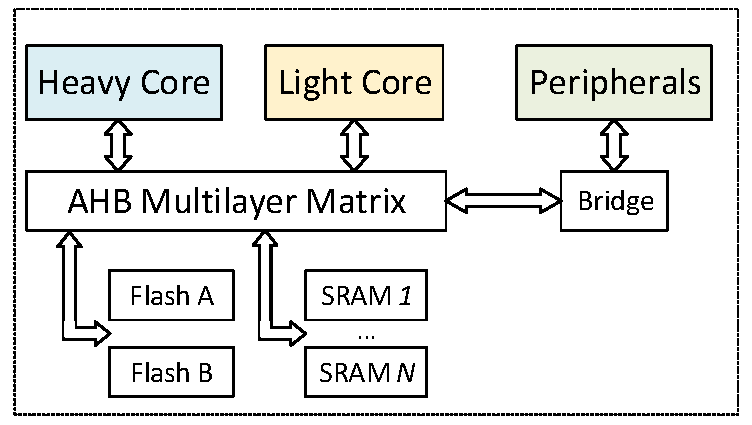
\includegraphics[scale=1]{./figures/system_model}
%  \caption{Hardware Architecture of proposed dual-core platform.}
%  \label{fig:system_model}
%\end{figure}
%As shown in Figure~\ref{fig:system_model}, the platform consists of two cores featuring the same ISA. The first core has been designed under the worst-case design margins, whereas the second one has been implemented to work under more relaxed operating conditions. In this semester thesis, we call the first core \emph{Heavy Core (HC)} and the second one \emph{Light Core (LC)}. The \emph{HC} is guaranteed to work at its maximum frequency (\emph{$F_{max}$}) with a probability of \emph{100\%}. On the other hand, the \emph{LC} might not always be able to reach the \emph{$F_{max}$}, but it is guaranteed to work at a frequency \emph{$F_{LC} \leq F_{max}$}, independently of the operating conditions. Moreover, the \emph{LC} is much more energy-efficient, because of its relaxed design margins, which means that when the two cores operate at the same frequency, the LC consumes less energy. The presence of the \emph{HC} provides some minimum performance guarantees and by offloading tasks to the \emph{LC}, we can improve substantially the energy consumption of the platform.\par


\begin{figure}[!tbp]
	\centering
	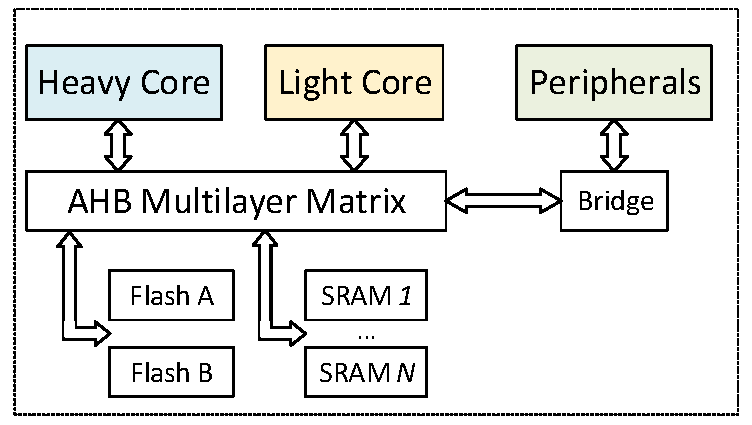
\includegraphics[width=0.7\linewidth]{./figures/system_model}
	\caption{Architecture of proposed dual-core platform.}
	\label{fig:system_model}
\end{figure}

\noindent\textbf{Power Model: }The system power consumption can be divided into three main components: the power consumption of the HC ($P_\mathrm{HC}$), the power consumption of the LC ($P_\mathrm{LC}$) and the power consumption of the system peripherals ($P_\mathrm{Sys}$). Due to reduced design margins, LC is more energy efficient compared to the HC. This implies that even when HC and LC operate at the same frequency, $P_\mathrm{LC}\leq P_\mathrm{HC}$. Each component has two different states: \emph{active} and \emph{sleep}. The sleep power of all components is non-negligible; however, it is constant. This constant factor is ignored in all power/energy computations in the remaining paper. Therefore, $P_\mathrm{X}=P_\mathrm{X,Active} - P_\mathrm{X,Sleep}\;, X\in\{\mathrm{HC}, \mathrm{LC}, \mathrm{SYS}\}$. The peripherals can be put into sleep only when both cores are in sleep state. 
%It is assumed that $P_\mathrm{Sys}$ is comparable to $P_\mathrm{HC}$. 
Formally, we focus on Heavy-Light platforms that operate under the following three conditions:\\
\textbf{Condition 1}: $F_\mathrm{HC}\geq F_\mathrm{LC}\geq \displaystyle\frac{ F_\mathrm{HC}}{2}$\\\\
\textbf{Condition 2}: $\displaystyle\frac{F_\mathrm{LC}}{P_\mathrm{LC}}\geq \displaystyle\frac{F_\mathrm{HC}}{P_\mathrm{HC}}$\\\\ 
\textbf{Condition 3}: $P_{\mathrm{HC}}\leq P_{\mathrm{LC}}+ P_{\mathrm{Sys}}$\\\\
%where: $P_\mathrm{X}=P_\mathrm{X,Active} - P_\mathrm{X,Sleep}\;, X\in\{\mathrm{HC}, \mathrm{LC}, \mathrm{SYS}\}$\\\\
Condition 1 emphasizes that LC might have performance penalty, due to its relaxed design margins. Condition 2 implies that LC is more energy efficient compared to HC, given that sleep powers are much smaller compared to active powers. Finally, condition 3 states that the power consumption of the peripherals is comparable to the power consumption of the HC. Previous works have shown that low power MCU platforms satisfy these conditions \cite{Gomez1, Fuks}.

\noindent\textbf{Task Model: }Applications consist of a set of \textit{n} periodic and independent tasks. It is assumed that all tasks have the same period $D$. Furthermore, it is assumed that all tasks are atomic units of execution; thus, preemptions and migrations are not allowed. This is a fairly restrictive assumption; however, it is realistic for deeply low power MCU platforms. $C_i$ is used to denote the computation cycles of task $i$.


%Studies have shown that in power-constrained MCU platforms, $E_{Sys}$ is comparable to $E_{HC}$. Therefore, our proposed solutions try to improve the energy consumption by minimizing the active time of the peripherals ($A_{SYS}$), as shown in Figure~\ref{fig:comparison}.
%\begin{figure}[!htbp]
%  \centering
%  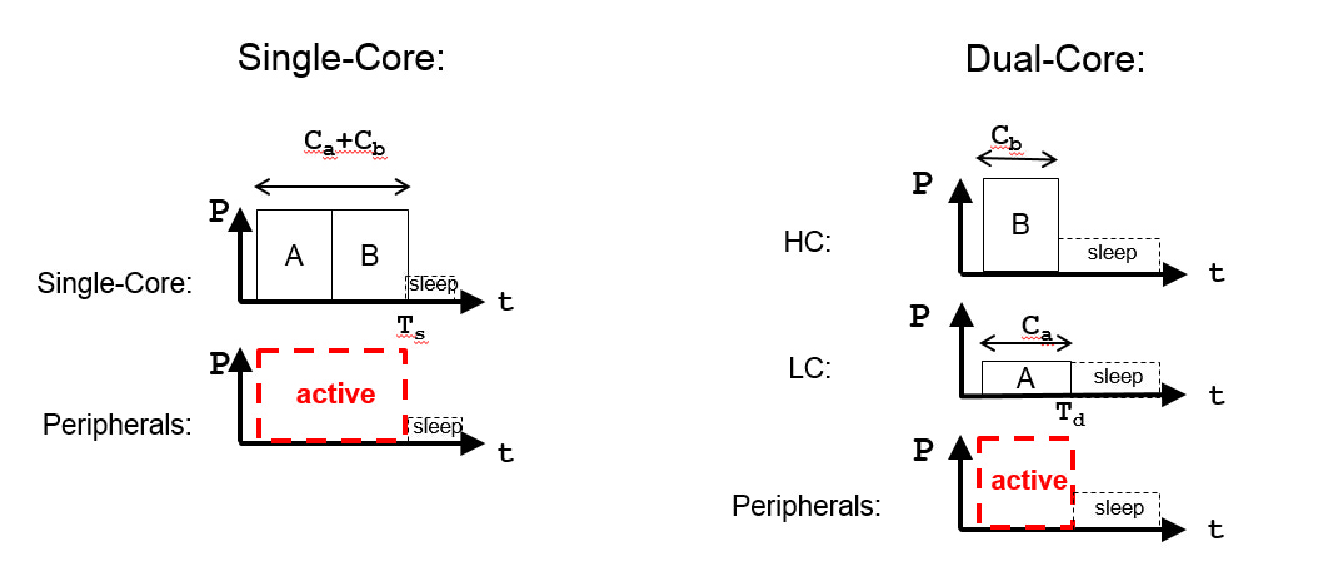
\includegraphics[width=\linewidth]{./figures/Comparison}
%  \caption{Comparison of a single-core and the proposed dual-core platform.}
%  \label{fig:comparison}
%\end{figure}

%\par
%The main advantages of the proposed architecture compared to the alternatives are the homogenous ISA and the energy efficiency offered by the \emph{LC}. This is in contrast to the modern dual-core MCU platforms which exploit the architectural heterogeneity in order to decrease the energy consumption. Due to architectural heterogeneity, the coprocessor cannot run the same applications as the main processor, rendering the platform inflexible. Dynamic allocation policies cannot be applied and any parallelization scheme has to be applied statically at design time. However, this is not a problem for the proposed architecture, as the two cores have the same ISA and thus they can allow more complex task allocation algorithms and parallelization schemes.\par



\section{Theoretical Results} \label{theory}
Since all tasks are atomic and have same deadline/period, the scheduling problem reduces to partitioning tasks to HC and LC with the objective of minimizing makespan or minimizing energy consumption. As we will see later in this section, for certain task and system configurations, these two objectives are conflicting. However, in most scenarios, these two objectives lead to the same solution i.e. minimizing makespan also minimizes energy. Formally, we can state the following optimization formulation:
\begin{figure}[h]
\hrulefill\\
\textbf{Variables:}
\begin{equation*}
\alpha_{i,X}=\begin{cases}1,&\mbox{if task ${i}$ is assigned to core $X\in\{\mathrm{HC, LC}\}$ }\\0,&\mbox{otherwise}
\end{cases}
\end{equation*}
\textbf{Objectives:}
\begin{align*}
\text{Obj 1: }& \text{Minimize} \big\{\max\{A_\mathrm{HC}, A_\mathrm{LC}\}\big\}\numberthis\label{equ:obj1}\\
\text{Obj 2: }& \text{Minimize} \big\{P_\mathrm{HC}A_\mathrm{HC}  + P_\mathrm{LC}A_\mathrm{LC} + P_\mathrm{Sys}A_\mathrm{sys}\big\}\numberthis\label{equ:obj2}\\
\text{where: }&A_\mathrm{X}=\sum_{1\leq i\leq n}\frac{\alpha_{i,\mathrm{X}}\cdot C_i}{F_X}\;, X\in\{\mathrm{HC}, \mathrm{LC}\}\\
&A_\mathrm{Sys}=\max\{A_\mathrm{HC}, A_\mathrm{LC} \}  
\end{align*}
\textbf{Constraints:}\\ \vspace{-1em}
\begin{align}
\sum_{X\in\{\mathrm{HC}, \mathrm{LC}\}}\alpha_{i,X}=1\qquad\forall  1\leq i\leq n\\
\max\{A_\mathrm{HC}, A_\mathrm{LC}\}\leq D
\end{align}
\hrulefill
\caption{Mixed Integer Linear Programming (MILP) formulation for the partitioning phase.}
\label{fig:miqcp}
\end{figure}

Objective 1 is minimizing makespan of the application while objective 2 is minimizing the energy consumption during one period $D$. The constraints specify that each task must be assigned to the HC or LC and that the application's makespan must be less than $D$. 

In the following section, we present theoretical results assuming that task-to-core partitioning is fixed/given. Later we will combine these theoretical results with a partitioning heuristic to propose our energy/performance oriented schemes.
Assuming fixed partitioning, we get two \textit{task bins} of possibly different sizes. We denote the total computation cycles of all tasks in the large bin  and small bin by $C_\mathrm{Lg}$ and $C_\mathrm{Sm}$ respectively ($C_\mathrm{Lg}\geq C_\mathrm{Sm}$). We also use an auxiliary variable $\Delta=\frac{C_{\mathrm{Lg}}-C_{\mathrm{Sm}}}{C_{\mathrm{Lg}}+C_{\mathrm{Sm}}}$ to quantify the imbalance between bins. $\Delta=0$ when both bins are equal and it approaches 1 as the imbalance between bins increases. Now we study the characteristics of task partitioning which minimizes makespan/energy. 

\begin{theorem}\label{thm:delta_opt}
The makespan and the energy consumption are simultaneously minimized when $\Delta=\Delta_\mathrm{opt}$, where:
\begin{equation}\label{equ:deltaopt}
\Delta_\mathrm{opt}=\frac{F_\mathrm{HC}-F_\mathrm{LC}}{F_\mathrm{HC}+F_\mathrm{LC}}\;
\end{equation}
 and the large/small task bins are executed in HC/LC respectively.
\end{theorem}
\noindent\textbf{Proof:} When $\Delta=\Delta_\mathrm{opt}$, $\frac{C_\mathrm{HC}-C_\mathrm{LC}}{C_\mathrm{HC}+C_\mathrm{LC}} =\frac{F_\mathrm{HC}-F_\mathrm{LC}}{F_\mathrm{HC}+F_\mathrm{LC}}$. This can be algebraically reduced to $\frac{C_\mathrm{Lg}}{F_\mathrm{Lg}} = \frac{C_\mathrm{Sm}}{F_\mathrm{Sm}}$. L.H.S is $A_\mathrm{HC}$ when HC executes the large task bin and R.H.S is $A_{LC}$ when LC executes the small task bin. Therefore, the active times of both cores are equal. Increasing the computation cycles of LC or HC, by shifting tasks, would increase the corresponding active time; thus increasing makespan. Therefore $\Delta=\Delta_\mathrm{opt}$ leads to the optimal makespan.
Now, we prove that $\Delta=\Delta_\mathrm{opt}$ with HC/LC executing large/small task bins also minimizes energy. Let us suppose that $A^*$ represents the optimal value of makespan. For this value, the energy consumption of the system during one period $D$ is: 
\begin{equation*}
E^*=A^*\cdot (P_\mathrm{HC} + P_\mathrm{LC}+ P_\mathrm{Sys})
\end{equation*}
Now suppose that from this optimal scenario, $0< x\leq A^*\cdot F_\mathrm{LC}$ computation cycles are shifted from the LC to HC. The new energy consumption is:
\begin{equation*}
E_1=(A^*+ \frac{x}{F_\mathrm{HC}})(P_\mathrm{HC} + P_\mathrm{Sys})+ (A^*- \frac{x}{F_\mathrm{LC}})  \cdot P_\mathrm{LC}
\end{equation*} 
Substracting $E^*$ from $E_1$, we get $x/F_\mathrm{HC}\cdot(P_\mathrm{HC}+P_\mathrm{Sys}) - x/F_\mathrm{LC}\cdot P_\mathrm{LC}$; which is always positive due to condition 2. Therefore, $E_1\geq E^*.$ 

Conversely, now suppose that from this optimal scenario, $0< x\leq A^*\cdot F_\mathrm{HC}$ computation cycles are shifted from the HC to LC. The new energy consumption is:
\begin{equation*}
E_2= (A^*- \frac{x}{F_\mathrm{HC}})  \cdot P_\mathrm{HC} +  (A^*+ \frac{x}{F_\mathrm{LC}})(P_\mathrm{LC} + P_\mathrm{Sys}) 
\end{equation*} 
Subtracting $E^*$ from $E_2$, we get $x/F_\mathrm{LC}\cdot(P_\mathrm{LC}+P_\mathrm{Sys}) - x/F_\mathrm{HC}\cdot P_\mathrm{LC}$; which is always positive due to conditions 1 and 3. Therefore, $E_2> E^*$. Consequently, $E^*$ is the minimum possible energy consumption for a given task-set. \qed

%The remaining section studies how tasks should be executed when optimal task partitioning ($\Delta=\Delta_\mathrm{opt}$) cannot be achieved. %when $\Delta\neq\Delta_{\mathrm{opt}}$ and the energy performance tradeoffs thereof. 
%From this point forward, we assume that $\Delta$ (and therefore the partitioning of tasks to bins) is given/fixed. 
Given fixed partitions, we can execute tasks in the following ways:
\begin{enumerate}
\item \textit{Scenario 1}: Large task bin executed on HC and small task bin executed on LC.
\item \textit{Scenario 2}: Small task bin executed on HC and large task bin executed on LC.
\item \textit{Scenario 3}: Both task bins executed on HC. 
\item \textit{Scenario 4}: Both task bins executed on LC. 
\end{enumerate}
We now study the conditions under which these execution scenarios are performance/energy optimal.

\begin{theorem}\label{thm: parallel-perf}
Executing large task bin on HC and small task bin on LC (Scenario 1) is always performance optimal. 
\end{theorem}
\noindent \textbf{Proof:} It is trivial to prove that scenario 1 has lower makespan compared to scenario 2 and scenario 3 has lower makespan compared to scenario 4. We will now prove that Scenario 1 outperforms Scenario 3. i.e. scenario 1 makespan $\leq$ scenario 3 makespan:
\[
\max\{C_\mathrm{Lg}/F_{\mathrm{HC}}, \;C_\mathrm{Sm}/F_{\mathrm{LC}} \}\leq (C_\mathrm{Lg}+C_\mathrm{sm})/F_\mathrm{HC} 
\]
The first term in the $\max$ is always less than RHS. Regarding the second term in the $\max$, $C_\mathrm{Sm}/F_{\mathrm{LC}}\leq $ RHS given condition 1.  \qed


We will now derive conditions for an \textit{energy optimal} scheme. The total energies for the four scenarios are calculated using following equations:  
\begin{align*}
E_{\mathrm{Total},1} =& P_{\mathrm{HC}}\cdot C_\mathrm{Lg}/F_\mathrm{HC} + P_{\mathrm{LC}}  \cdot C_\mathrm{Sm}/F_\mathrm{LC}\\
&+P_{\mathrm{Sys}}\cdot \max(C_\mathrm{Lg}/F_\mathrm{HC},\;C_\mathrm{Sm}/F_\mathrm{LC})\\ 
E_{\mathrm{Total},2} =& P_{\mathrm{HC}}\cdot C_\mathrm{Sm}/F_\mathrm{HC} + (P_{\mathrm{LC}}+ P_{\mathrm{Sys}})  \cdot C_\mathrm{Lg}/F_\mathrm{LC}\\
E_{\mathrm{Total},3} =& (P_{\mathrm{HC}} + P_{\mathrm{Sys}})\cdot (C_\mathrm{Lg}+ C_\mathrm{Sm})/F_\mathrm{HC}\\
E_{\mathrm{Total},4} =& (P_{\mathrm{LC}} + P_{\mathrm{Sys}})\cdot (C_\mathrm{Lg}+ C_\mathrm{Sm})/F_\mathrm{LC}
\end{align*}
\begin{theorem}\label{thm:parallel}
It is always energy optimal to parallelize workload.
\end{theorem}
\noindent\textbf{Proof:} We first prove that $E_\mathrm{Total, 1}\leq E_\mathrm{Total, 3}$. We then prove that $E_\mathrm{Total, 2}\leq E_\mathrm{Total, 4}$, proving that parallelizing workload always leads to lower energy consumption.  
\begin{align*} 
 E_{\mathrm{Total},1}-E_{\mathrm{Total},3}=& P_{\mathrm{LC}} \cdot \frac{C_\mathrm{Sm}}{F_\mathrm{LC}} + P_{\mathrm{Sys}}\cdot \max(\frac{C_\mathrm{Lg}}{F_\mathrm{HC}},\;\frac{C_\mathrm{Sm}}{F_\mathrm{LC}}) 
\\&- P_{\mathrm{HC}} \cdot \frac{C_\mathrm{Sm}}{F_\mathrm{HC}}-P_{\mathrm{Sys}}\cdot \frac{C_\mathrm{Lg}+C_\mathrm{Sm}}{F_\mathrm{HC}}
\end{align*}

By Theorem~\ref{thm: parallel-perf}, $\max\{C_\mathrm{Lg}/F_{\mathrm{HC}}, \;C_\mathrm{Sm}/F_{\mathrm{LC}} \}\leq \frac{C_\mathrm{Lg}+C_\mathrm{sm}}{F_\mathrm{HC}}$. Therefore:
\[ 
 E_{\mathrm{Total},1}-E_{\mathrm{Total},3}\leq P_{\mathrm{LC}} \cdot \frac{C_\mathrm{Sm}}{F_\mathrm{LC}}- P_{\mathrm{HC}} \cdot\frac{C_\mathrm{Sm}}{F_\mathrm{HC}}
\]
R.H.S is always $\leq 0$ due to condition 2, therefore $E_\mathrm{Total, 1}\leq E_\mathrm{Total, 3}$. We now prove $E_\mathrm{Total,2}\leq E_\mathrm{Total,4}$:
\begin{equation*}
\begin{split}
E_\mathrm{Total,2}-E_\mathrm{Total,4}=P_{\mathrm{HC}}\cdot \frac{C_\mathrm{Sm}}{F_\mathrm{HC}} - (P_{\mathrm{LC}}+P_{\mathrm{Sys}})  \cdot \frac{C_\mathrm{Sm}}{F_\mathrm{LC}} 
\end{split}
\end{equation*}
R.H.S. $\leq$ 0 if conditions 1 and 3 are valid. \qed

We now derive conditions where the scenario 1 and scenario 2 are energy optimal. 

%Note that for scenario 2, $P_{\mathrm{sys},A}$ is consumed for $A_{\mathrm{LC},2}$ because $A_{\mathrm{LC},2}\geq A_{\mathrm{HC},2}$ irrespective of the value of $\Delta$.
\begin{theorem}\label{thm:case1vscase2}
$E_{\mathrm{Total},1}\leq E_{\mathrm{Total},2}$ \textbf{iff}: $\Delta\leq\max\{\Delta_\mathrm{opt},\; \Delta_\mathrm{diff}\}$, where:
\begin{equation}\label{equ:deltadiff}
\Delta_\mathrm{diff}=\frac{P_\mathrm{Sys} (F_\mathrm{HC}-F_\mathrm{LC})}{2 (F_\mathrm{LC}  P_\mathrm{HC} - F_\mathrm{HC} P_\mathrm{LC}) - P_\mathrm{Sys} (F_\mathrm{HC}-F_\mathrm{LC})} 
\end{equation}
\end{theorem}
\noindent\textbf{Proof:} We prove this for two cases: $\Delta\leq\Delta_\mathrm{opt}$ and $\Delta>\Delta_\mathrm{opt}$.\\
\textbf{Case 1:} $0\leq\Delta\leq \Delta_\mathrm{opt}$. In Scenario 1, $A_\mathrm{HC}\leq A_\mathrm{LC}$. Therefore, the active time of the system $A_\mathrm{Sys}=A_\mathrm{LC}=C_\mathrm{Sm}/F_\mathrm{LC}$. So:
\begin{align*}
E_\mathrm{Total, 1}-E_\mathrm{Total, 2}=&P_\mathrm{HC}(C_\mathrm{Lg}-C_\mathrm{Sm})/F_\mathrm{HC} \\& -(P_\mathrm{LC}+P_\mathrm{Sys})(C_\mathrm{Lg}-C_\mathrm{Sm})/F_\mathrm{LC}
\end{align*}
The positive term in this equation is never greater than the negative term due to conditions 1 and 3. Therefore $E_\mathrm{Total, 1}\leq E_\mathrm{Total, 2}\; \forall \; 0\leq\Delta\leq \Delta_\mathrm{opt}$. \\
\textbf{Case 2:} $\Delta> \Delta_\mathrm{opt}$. In Scenario 1, $A_\mathrm{HC}>A_\mathrm{LC}$. Therefore, the active time of the system $A_\mathrm{Sys}=A_\mathrm{HC}=C_\mathrm{Lg}/F_\mathrm{HC}$. We now find the condition where $E_\mathrm{Total, 1}-E_\mathrm{Total, 2}\leq 0$
\begin{align*}
P_\mathrm{HC}(C_\mathrm{Lg}-C_\mathrm{Sm})/F_\mathrm{HC} - P_\mathrm{LC}(C_\mathrm{Lg}-C_\mathrm{Sm})/F_\mathrm{LC}\\
-P_\mathrm{Sys}\cdot C_\mathrm{Lg}(F_\mathrm{HC}-F_\mathrm{LC})/(F_\mathrm{HC}\cdot F_\mathrm{LC})&\leq 0\\ 
\implies \frac{P_\mathrm{HC}}{F_\mathrm{HC}}-\frac{P_\mathrm{LC}}{F_\mathrm{LC}}-P_\mathrm{Sys}\frac{C_\mathrm{Lg}}{{C_\mathrm{Lg}-C_\mathrm{Sm}}}\frac{F_\mathrm{HC}-F_\mathrm{LC}}{F_\mathrm{HC}\cdot F_\mathrm{LC}}&\leq 0
\end{align*}
Substituting $\frac{C_\mathrm{Lg}}{{C_\mathrm{Lg}-C_\mathrm{Sm}}} = \frac{\Delta+1}{2\Delta}$ and solving to $\Delta$ leads to the R.H.S of \eqref{equ:deltadiff}. Combining case 1 and case 2 conditions proves the theorem.\qed

\subsection{Task Allocation Policies}
Firstly, all tasks are partitioned with the objective of making $\Delta=\Delta_\mathrm{opt}=\frac{F_\mathrm{HC}-F_\mathrm{LC}}{F_\mathrm{HC}+F_\mathrm{LC}}$. We utilize a heuristic algorithm that does bin-packing of tasks to cores with the objective of $\Delta=\Delta_\mathrm{opt}$. Specifically, given a set of tasks and two uniform (non-identical) cores, assign tasks to cores such that makespan is minimized. This is a well studied $Q2||C_{\mathrm{max}}$ problem and is known to be NP-Hard. However, the Modified Longest Processing Time (MLPT) heuristic proposed in \cite{mlpt} solves this problem with an approximation ratio of 1.22. MLPT also has low complexity $O(n\log n +c)$ and therefore can be applied at runtime. The working of MLPT algorithm is summarized here for completeness:
\begin{enumerate}
	\item Sort all tasks in non-increasing order of their computation times.
	\item if $n\leq2$, assign tasks greedily such that their individual completion/finish time is minimized. 
	\item if $n\geq 3$, assign the first three (largest) tasks optimally such that their makespan is minimized. Assign the remaining tasks greedily such that their individual completion/finish time is minimized.
\end{enumerate}
Next, the task bins are executed using the following policies:
\begin{enumerate}
\item \emph{Delta Threshold Mapping-Makespan (DTM-M)}: Execute \textit{Large} task bin on the HC and \textit{Small} task bin on LC.
\item \emph{Delta Threshold Mapping-Energy (DTM-E)}: Execute \textit{Large} task bin on HC and \textit{Small} task bin on the LC if $\Delta \leq \max\{\Delta_\mathrm{opt},\;\Delta_\mathrm{diff}\}$ \textbf{OR} $\frac{C_\mathrm{Lg}}{F_\mathrm{LC}}\leq D$. %$\Delta_\mathrm{opt}$ and $\Delta_\mathrm{diff}$ are defined in equations \eqref{equ:deltaopt} and \eqref{equ:deltadiff} respectively. 
Do the converse otherwise. 
\end{enumerate}
The optimality of these approaches for a given partitioning has been proved in Theorem \ref{thm: parallel-perf} and \ref{thm:case1vscase2}. 

\begin{figure*}[!t]
	\centering
	\begin{subfigure}{.5\columnwidth}
		\centering
		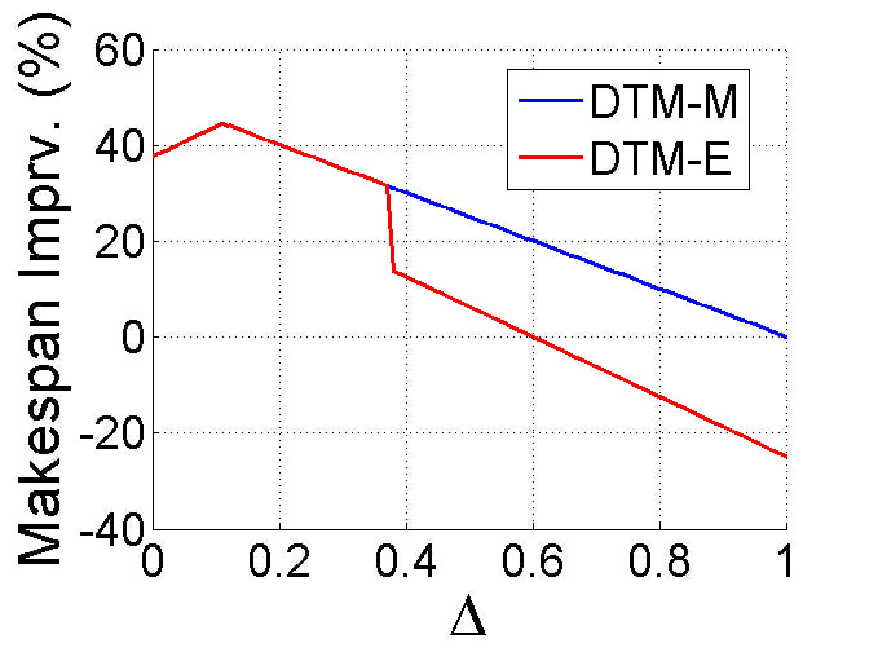
\includegraphics[width=\columnwidth]{./figures/flc_80_delta_makespan_theory}
		\caption{Makespan Simulation}
		\label{fig:Flc80-delta-makespan-theory}
	\end{subfigure}
	\begin{subfigure}{.5\columnwidth}
		\centering
		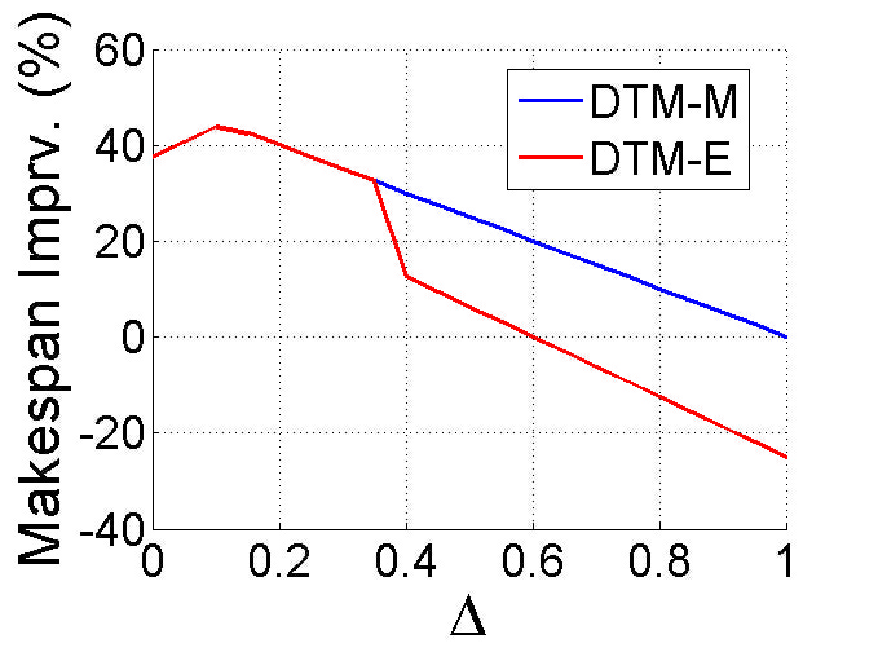
\includegraphics[width=\columnwidth]{./figures/flc_80_delta_makespan}
		\caption{Makespan Experiment}
		\label{fig:Flc80-delta-makespan}
	\end{subfigure}
	\begin{subfigure}{.5\columnwidth}
		\centering
		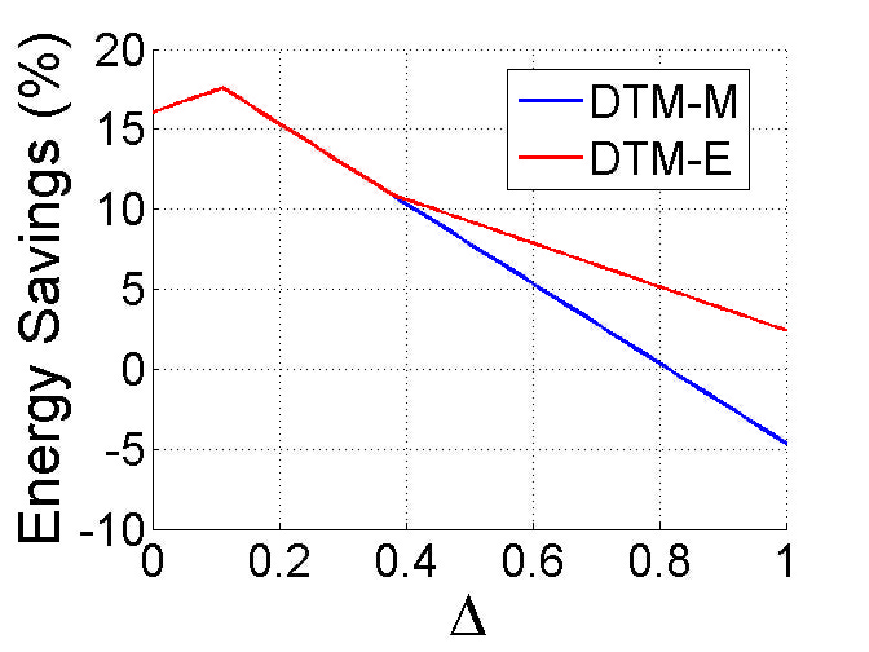
\includegraphics[width=\columnwidth]{./figures/flc_80_delta_energy_theory}
		\caption{Energy Simulation}
		\label{fig:Flc80-delta-energy-theory}
	\end{subfigure}
	\begin{subfigure}{.5\columnwidth}
		\centering
		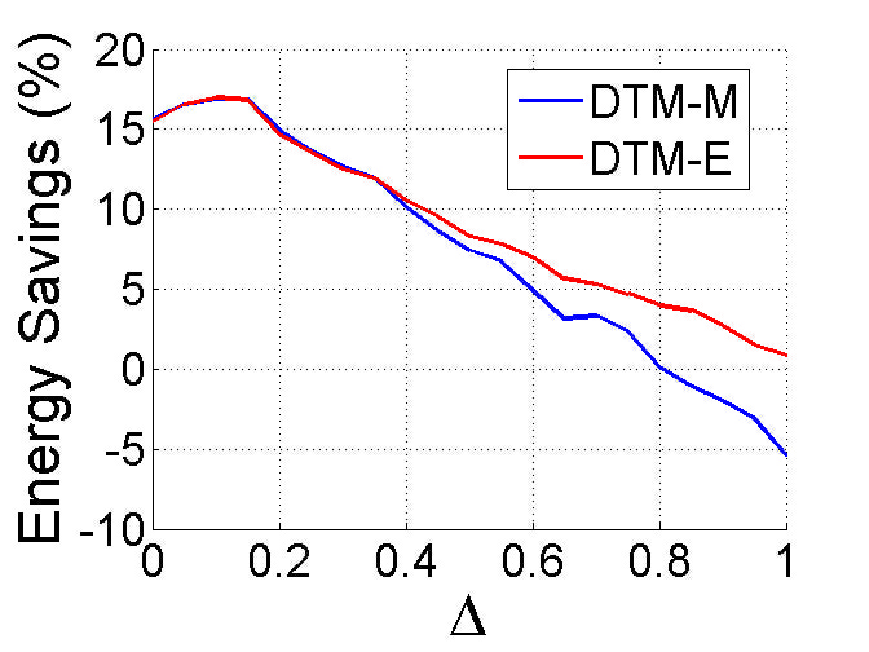
\includegraphics[width=\columnwidth]{./figures/flc_80_delta_energy}
		\caption{Energy Experiment}
		\label{fig:Flc80-delta-energy}
	\end{subfigure}
	\caption{Dynamic Threshold Mapping (DTM) Energy and Performance Results for $F_{LC} = 80 MHz$ and utilization = 50\%.}
	\label{fig:Flc80-delta}
\end{figure*}

\section{Evaluation Methodology} \label{results}
%%%%%%%%%%%%%%%%%%%%%%%%%%%%%%%%%%%%%%%%%%%%%%%%%%%%%%%%%%%%%%%%%%%%%%%
%%%%%%%%%%%%%%%%%%%%%%%%%%%%%%%%%%%%%%%%%%%%%%%%%%%%%%%%%%%%%%%%%%%%%%%
%%%%%                                                                 %
%%%%%     <file_name>.tex                                             %
%%%%%                                                                 %
%%%%% Author:      <author>                                           %
%%%%% Created:     <date>                                             %
%%%%% Description: <description>                                      %
%%%%%                                                                 %
%%%%%%%%%%%%%%%%%%%%%%%%%%%%%%%%%%%%%%%%%%%%%%%%%%%%%%%%%%%%%%%%%%%%%%%
%%%%%%%%%%%%%%%%%%%%%%%%%%%%%%%%%%%%%%%%%%%%%%%%%%%%%%%%%%%%%%%%%%%%%%%\\

In this section, we present our experimental results in order to validate our theoretical findings and prove the merits of the Heavy-Light architecture. First, we will use randomized task sets to compare an energy optimal partitioning to state-of-the-art heuristics with and without DTM. Afterwards, we will use fixed partitions to evaluate our DTM algorithms, with both synthetic and real-world benchmarks.

\noindent\textbf{Hardware Testbed:}
Since the Heavy-Light platform is not commercially available, we can only emulate heavy light behavior using a commercially available dual-core platform. In this work, we use the LPCXpresso54102 platform, which consists of a performance-oriented Cortex M4 core and an energy-efficient Cortex M0 core. 
The only difference with a Heavy-Light platform is that the LPC has heterogeneous microarchitectures. In order to emulate a Cortex M4-based Heavy-Light platform, we characterize our applications by running them on the M4 at different frequencies, recording their execution times and energy. To test our task allocation policies, the M0 is configured to consume either the same clock cycles or energy as a Light M4 core running a task at a given $F_{LC}$ would, depending on the experiment. Tasks are executed in bare metal and the communication between cores is minimal, so any overheads are negligible when compared to task execution lengths.

\begin{table}[!t]
	\centering
	\caption{Estimated Power Values for Heavy-Light Platform}
	\label{tab:power_numbers_exp}
	\begin{tabular}{|c|c|c|c|} \hline
		\textbf{Component} & $\mathbf{P_\mathrm{\mathbf{Active}}}$ & $\mathbf{P_\mathrm{\mathbf{Sleep}}}$ & $\mathbf{P_\mathrm{\mathbf{Difference}}}$\\ 
		\hline
		Heavy (100MHz)& 22.1 mW & 2 mW & 20.1 mW\\
		\hline
		Light (100MHz) & 15.5 mW & 1.4 mW & 14.1 mW\\ 
		\hline
		Light (80MHz) & 12.1 mW & 1.4 mW & 10.7 mW\\ 
		\hline
		Peripherals & 16.6 mW & 2 mW & 14.6 mW\\ 
		\hline
	\end{tabular}
\end{table}

%For emulation, the M4 is treated as HC and the M0 is treated as the LC. In the actual platform, both cores run at the same frequency of $100MHz$.
The makespan and power consumption of the platform is logged using a National Instruments USB-6216 Data Acquisition board. Table~\ref{tab:power_numbers_exp} shows the power consumption of the HC and LC at 100MHz. The former is the measured power consumption of the LPC's Cortex M4, and the ladder is the estimate of an M4 LC with reduced power density. The power consumption of the LC scales linearly with its operating frequency, $F_{LC}$.

The makespan improvement and energy savings from the Heavy-Light Platform are always compared to a Cortex M4 based, single-core platform. 
%Experimentally, the energy consumption of the HC is always measured. However, the energy consumption of the LC at different operating frequencies can only be estimated; since the LPC platform does not allow us to change the frequency of HC and LC cores independently. 
To allow a fair comparison, the energy consumption values for single-core were acquired by executing all the tasks on the HC and subtracting the energy consumed by the LC, which is kept in sleep state.

%Both cores can run at a maximum frequency of $100 MHz$. %We modified the software running on the M0 such that either the execution time or energy consumption of tasks, depending on what was being measured, would match that of an actual LC. This required a per-characterization step, during which the execution time and power consumption of tasks running on the HC, at both maximum and reduced frequencies, were recorded.

%We first study the performance of MLPT heuristic as a function of the number of randomly generated tasks. 
%As a first step, we conducted a simulation in Matlab in order to study the correlation between $\Delta$ and the total number of tasks partitioned to the two task bins.
We first compare the performance of DTM-E to a state-of-the-art heuristic called LP+BP. As was previously mentioned in Section~\ref{related}, the heuristic presented in \cite{Paterna} uses a Linear Programming (LP) formulation and a modified Bin Packing (BP) algorithm to reduce the energy consumption in accelerators. %\textbf{Add some additional lines here explaining LP+BP}.


 %In this algorithm, the total number of tasks and the sum of computation cycles can be set as parameters. Computation times of individual tasks are assigned randomly. In Figure~\ref{fig:delta-tasks}, we compare the performance of MLPT with an optimal task allocation policy; for different number of tasks and different values of $F_\mathrm{LC}$. As shown in Figure~\ref{fig:delta-tasks}, MLPT performs close to optimal for all simulations. Furthermore, $\Delta$ approaches $\Delta_\mathrm{opt}$ ($|{\Delta - \Delta_\mathrm{opt}}|_\mathrm{avg}\rightarrow 0$) for a reasonable number of randomly generated tasks ($\geq 10$). From this result, we can conclude that when the number of tasks $\geq 10$, MLPT approaches to the optimal task partition; which minimizes both makespan and energy consumption (Theorem~\ref{thm:delta_opt}).
%Later on, we conduct experiments assuming that $\Delta$ is fixed/given. We evaluate both synthetic benchmarks and a real-world application. 

%The task allocation was done by using the MLPT \cite{mlpt} heuristic, which is suitable for performance-constrained devices. Figure ~\ref{fig:delta-tasks} shows the results for different values of $F_\mathrm{LC}$. We note that even for a low number of tasks the divergence between $\Delta$ and $\Delta_\mathrm{opt}$ is not extensive. Furthermore, for $n \geq 10$ the convergence to $\Delta_\mathrm{opt}$ is almost absolute.\par
%\vspace{-1em}
%\begin{figure}[!hbtp]
%\centering
%  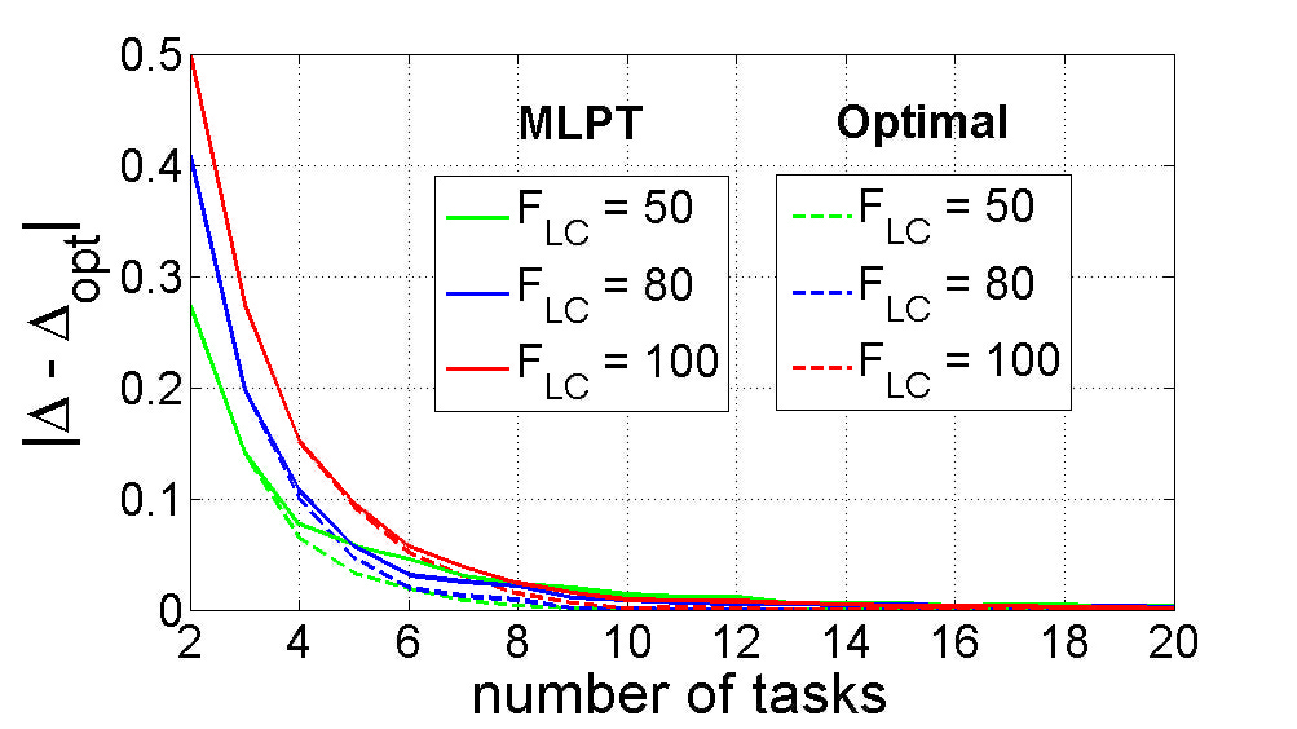
\includegraphics[width=0.8\columnwidth]{./figures/delta-tasks}
%  \caption{Correlation between $\Delta$ and the number of tasks}
%  \label{fig:delta-tasks}
%\end{figure}

\begin{figure}[!b]
	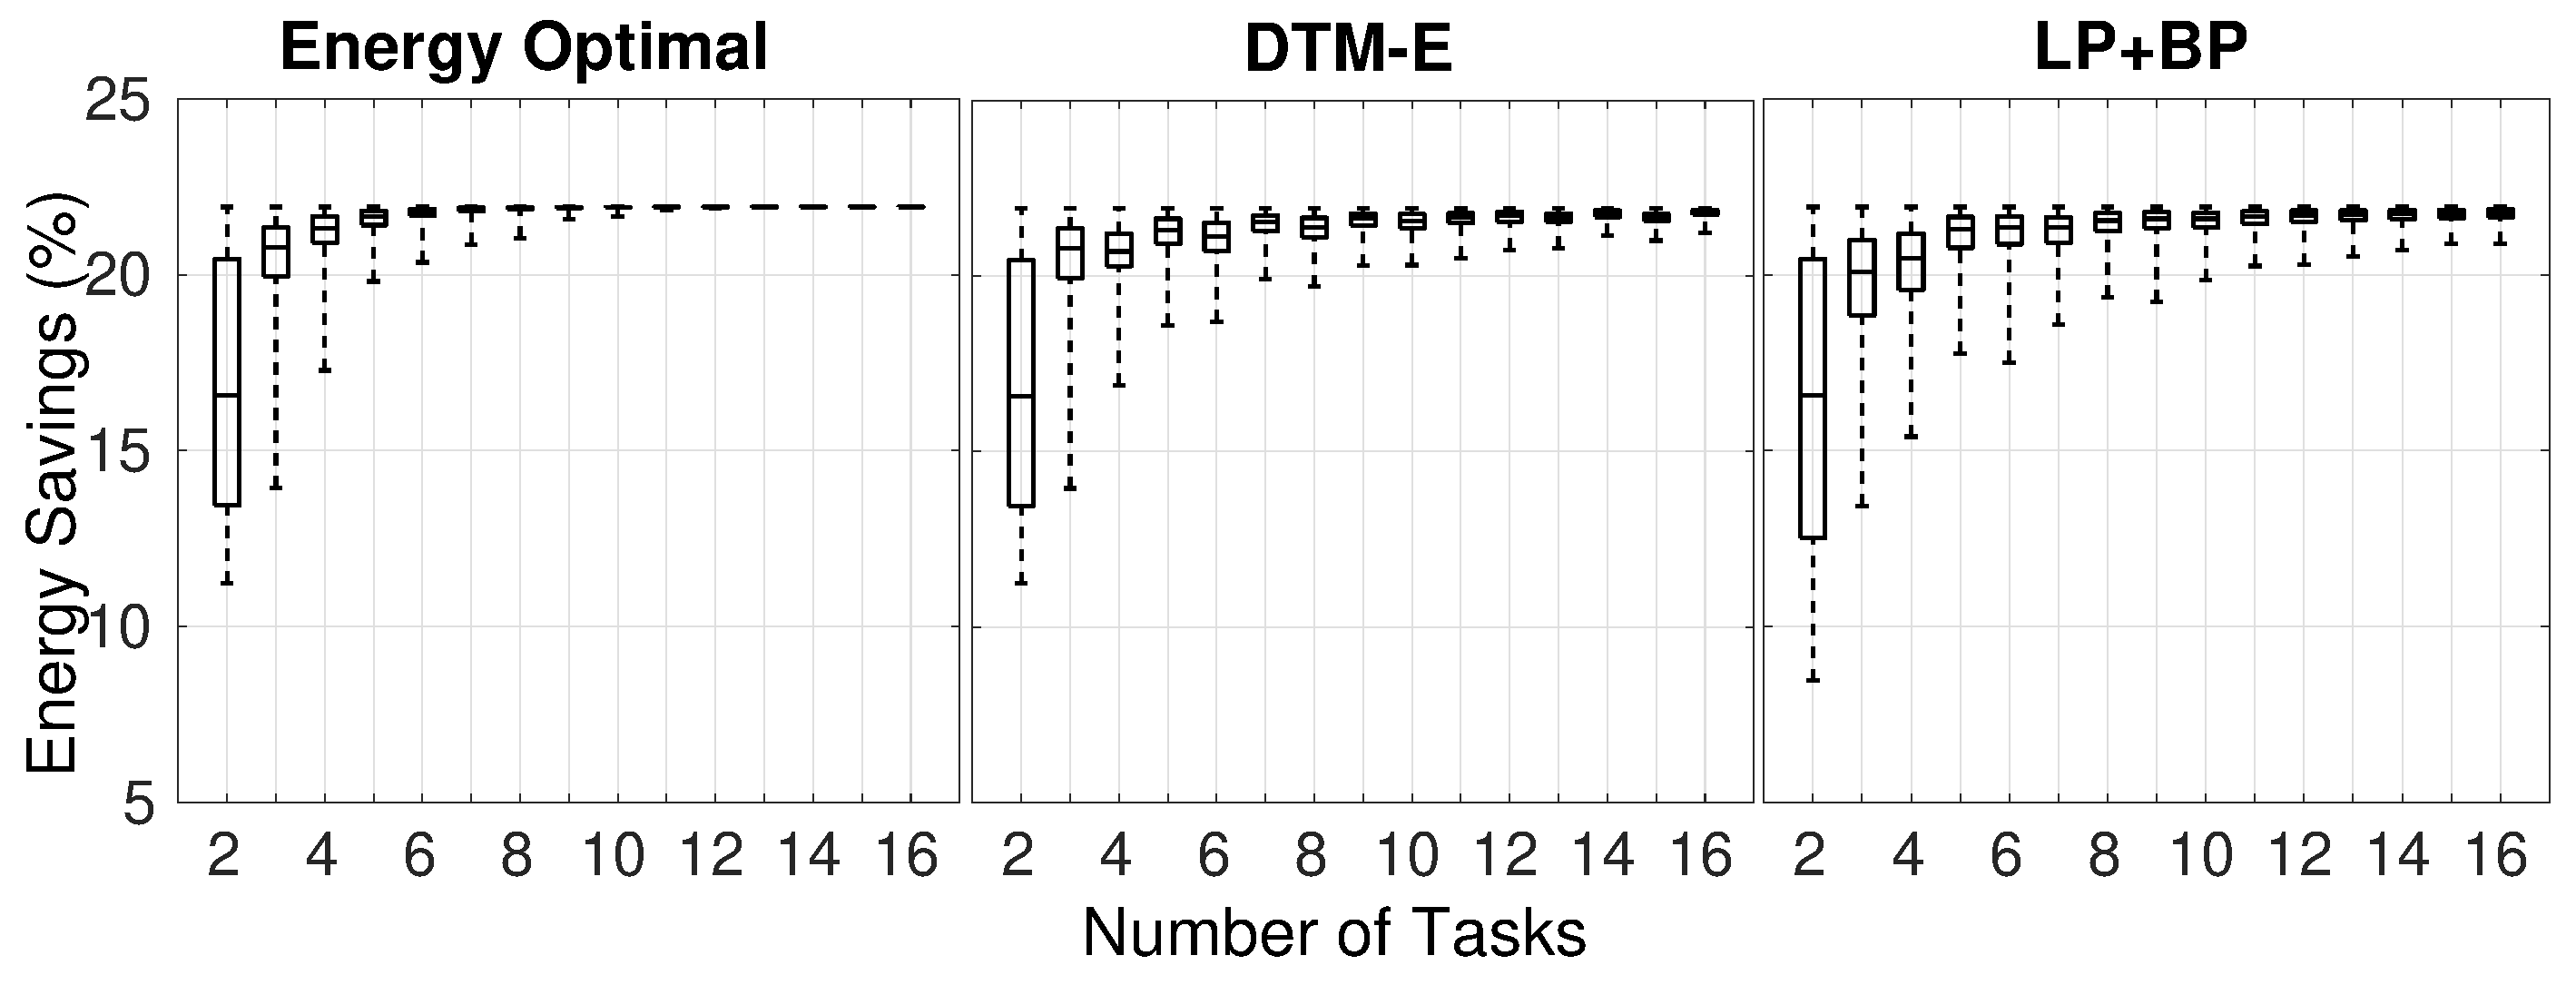
\includegraphics[width=\columnwidth]{./figures/opt_DTM_LPBP}
	\caption{Optimal vs DTM-E vs LP+BP}
	\label{fig:comparison}
\end{figure}

%\begin{figure}[!b]
%	\centering
%	\begin{subfigure}{.48\columnwidth}
%		\centering
%		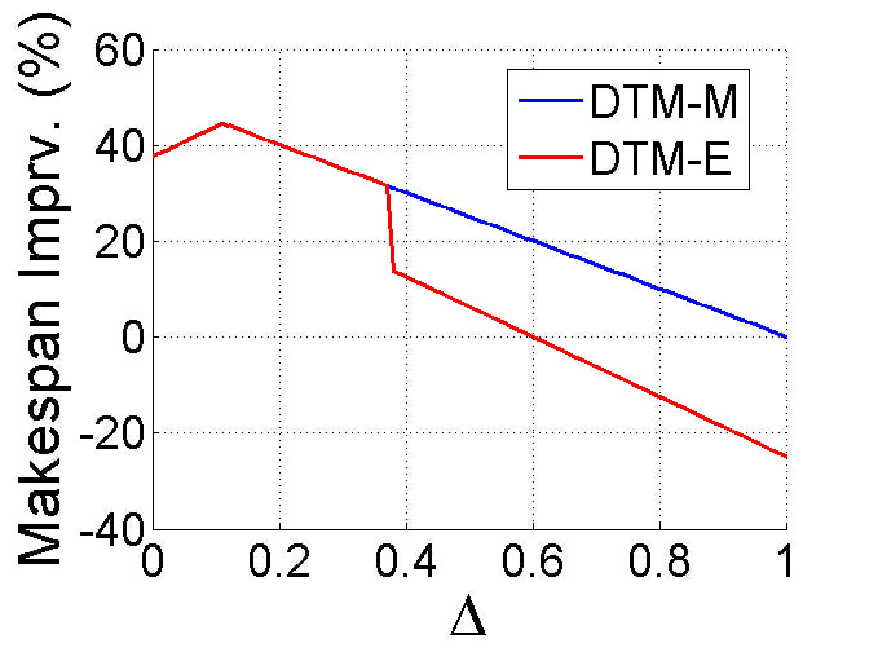
\includegraphics[width=\columnwidth]{./figures/flc_80_delta_makespan_theory}
%		\caption{Makespan Simulation}
%		\label{fig:Flc80-delta-makespan-theory}
%	\end{subfigure}
%	\begin{subfigure}{.48\columnwidth}
%		\centering
%		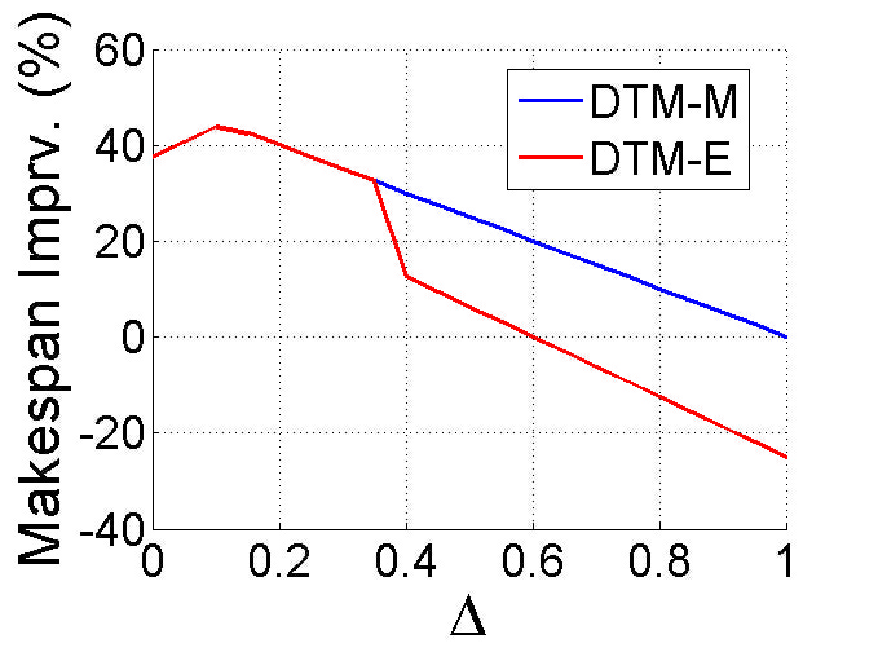
\includegraphics[width=\columnwidth]{./figures/flc_80_delta_makespan}
%		\caption{Makespan Experiment}
%		\label{fig:Flc80-delta-makespan}
%	\end{subfigure}
%	\caption{Makespan Results for $F_{LC} = 80 MHz$ and utilization = 50\%.}
%	\label{fig:flow}
%\end{figure}

\noindent\textbf{Comparison with LP+BP and Optimal mapping:}

To compare DTM-E approach, we generated 150000 random task-sets with up to 16 tasks and 100\% utilization. \emph{UUniFast}\cite{uunifast} algorithm is used to synthetically generate tasksets with fixed number of tasks. During this comparison, we assumed that $F_{HC} = 100MHz$ and $F_{LC} = 80MHz$, and considered the power consumption of the components as shown in Table~\ref{tab:power_numbers_exp}. By applying both the optimal formulation, DTM-E scheme and the LP+BP algorithm, we estimated the energy savings compared to a single-core using Matlab. The results can be seen in Figure~\ref{fig:comparison}. Firstly, note that the performance of DTM-E is near optimal. The mean and second/third quartile values are nearly identical for all simulation points. However, the fourth quartile values are marginally different. %Notice that, when the number of tasks is low (2, 3, 4), there are some tasksets which have negative energy savings. This may seem in conflict with our theoretical results (Specifically Theorem~\ref{thm:parallel}). However, this is not a contradiction because the single-core power we compare against has no sleep power for the LC. Therefore, the sleep power dissipation of the single core is lower compared to the sleep power of the Heavy-Light platform. This inherent difference in system efficiency leads to some corner cases where energy consumption of the dual core is higher compared to the energy consumption of the single core. 
While all schemes converge towards 22\% energy savings as the number of tasks increase, there is a clear difference for a low number of tasks between LP+BP and Optimal/DTM-E. We notice that although the mean values of all three schemes are similar, for low number of tasks, the worst case for LP+BP (fourth quartile) is significantly lower compared to the worst-case for DTM-E and optimal results. The difference stems from the fact that applications targeted by LP+BP exhibit a high degree of parallelism. In other words, when $\Delta$ is close to $\Delta_\mathrm{opt}$. If two task bins have significantly different sizes (leading to a high $\Delta$), the LP+BP algorithm is expected to have lower energy savings.  
 

%We notice that the mean energy savings for tasksets having two tasks is 11.0062, 11.0062 and 10.687 for opt, DTM-E and LP+BP respectively. Furthermore, we also notice a difference in average values for tasksets having three tasks (16.6395 vs 16.6323 vs 16.1795). However, in general, the difference becomes less as the number of tasks increase. This is because the difference stems from the fact that applications targeted by LP+BP exhibit a high degree of parallelism. In other words, when $\Delta$ is close to $\Delta_\mathrm{opt}$. If two task bins have significantly different sizes (leading to a high $\Delta$), the LP+BP algorithm can have lower energy savings.  

%\vspace{-1em}
%\begin{figure}[!htb]
%	\centering
%	\begin{subfigure}{.48\columnwidth}
%		\centering
%		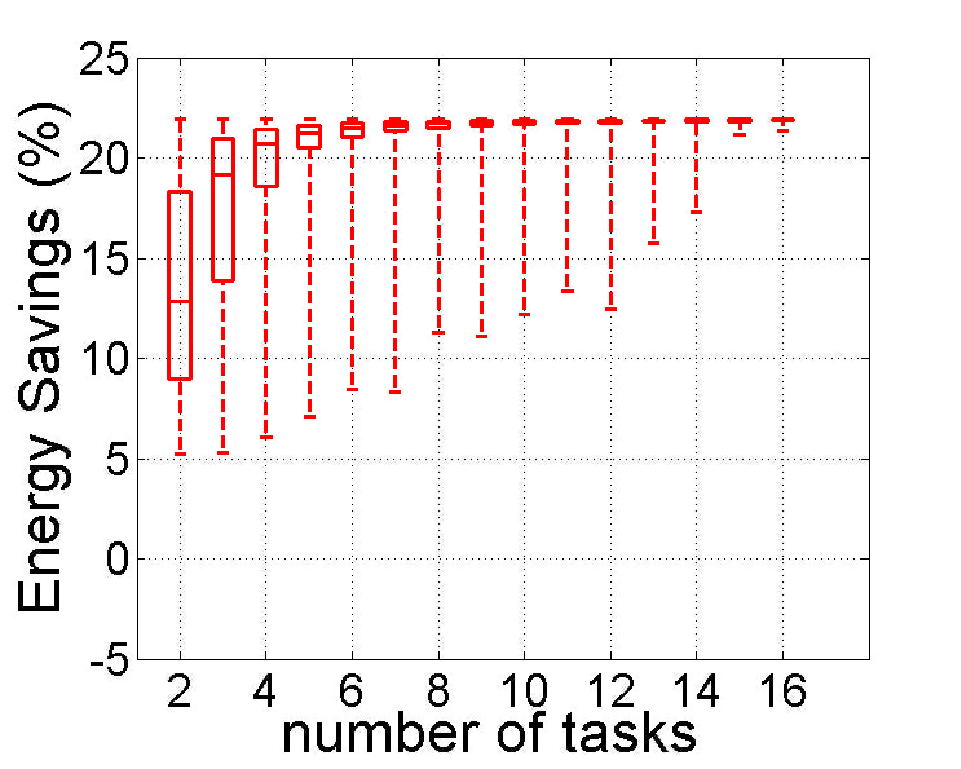
\includegraphics[width=\columnwidth]{./figures/energy_efficient}
%		\caption{DTM-E}
%		\label{fig:proposed_scheme}
%%%		\centering
%		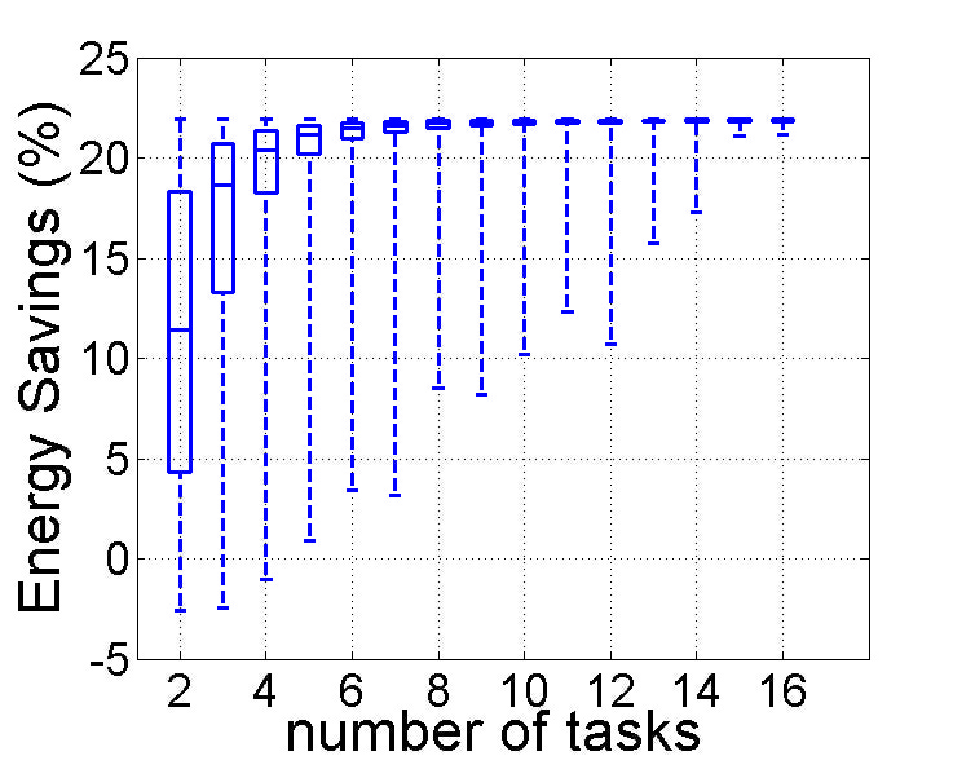
\includegraphics[width=\columnwidth]{./figures/lpbp}
%		\caption{LP+BP Algorithm\cite{Paterna}}
%		\label{fig:lpbp}
%	\end{subfigure}
%	\vspace{-0.05in}
%	\caption{Energy Savings for randomly generated task sets.}
%	\label{fig:comparison}
%\end{figure}

\noindent\textbf{Evaluation using Synthetic Benchmarks: }
The synthetic benchmark evaluation is used to quantify the effects of the single-core utilization and $\Delta$ on performance/energy improvement. For each utilization-$\Delta$ pair, we run 100 iterations of the application on the hardware test-bed, logging both the makespan and energy consumption of the Heavy-Light and single-core architectures. During these experiments, we also assumed $F_{HC} = 100$MHz and $F_{LC} = 80$MHz.\par

\begin{figure}[!b]
\centering
\begin{subfigure}{.48\columnwidth}
  \centering
  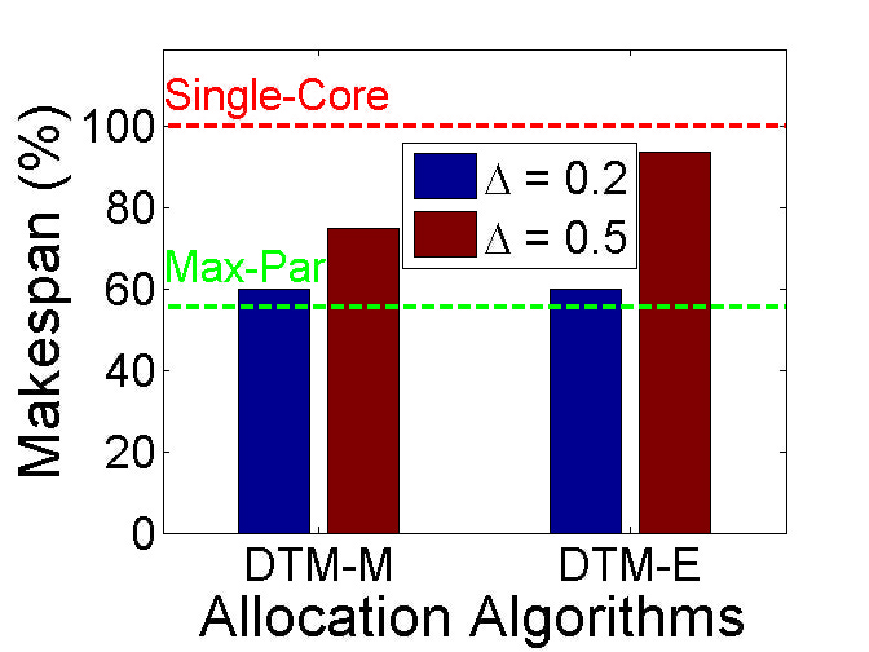
\includegraphics[width=\columnwidth]{./figures/flc_80_util_makespan}
  \caption{Makespan Experiment}
  \label{fig:Flc80-util-makespan}
\end{subfigure}
\begin{subfigure}{.48\columnwidth}
  \centering
  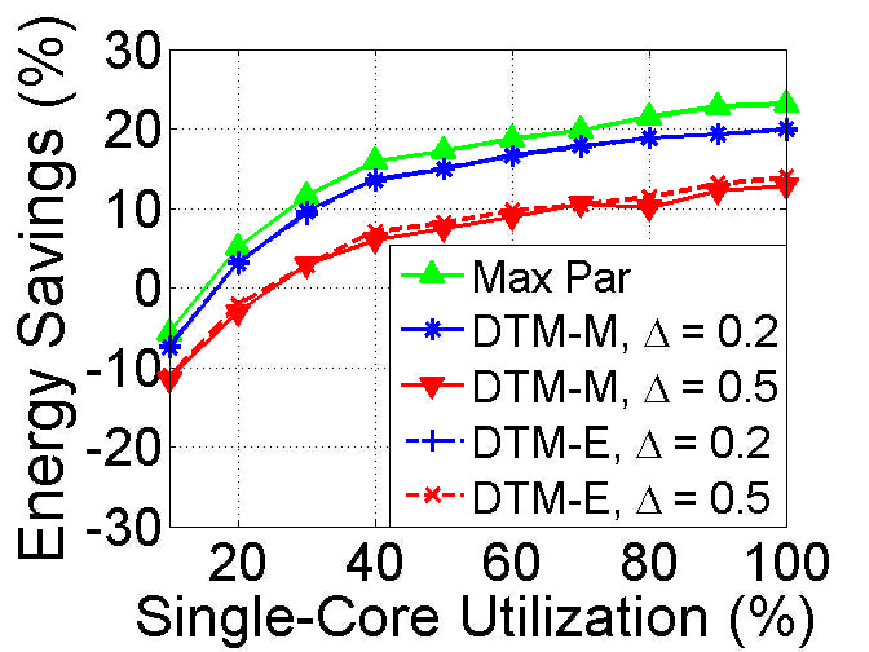
\includegraphics[width=\columnwidth]{./figures/flc_80_util_energy}
  \caption{Energy Experiment}
  \label{fig:Flc80-util-energy}
\end{subfigure}
\vspace{-0.05in}
\caption{Makespan and Energy Savings for $F_{LC} = 80 MHz$.}
\label{fig:Flc80-util}
\end{figure}
%\vspace{-0.1in}

%\begin{figure}[!b]
%	\centering
%	\begin{subfigure}{.48\columnwidth}
%		\centering
%		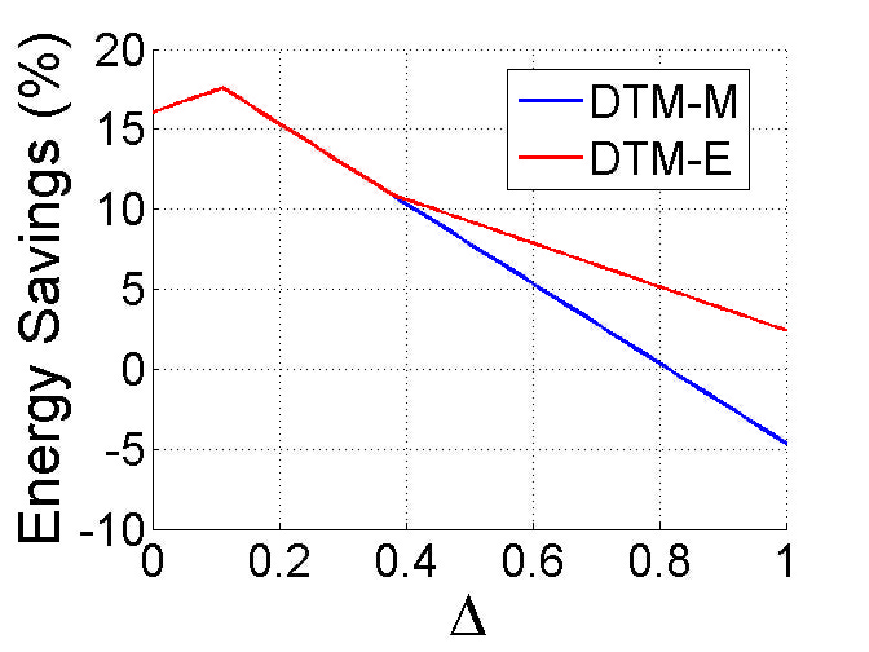
\includegraphics[width=\columnwidth]{./figures/flc_80_delta_energy_theory}
%		\caption{Energy Simulation}
%		\label{fig:Flc80-delta-energy-theory}
%	\end{subfigure}
%	\begin{subfigure}{.48\columnwidth}
%		\centering
%		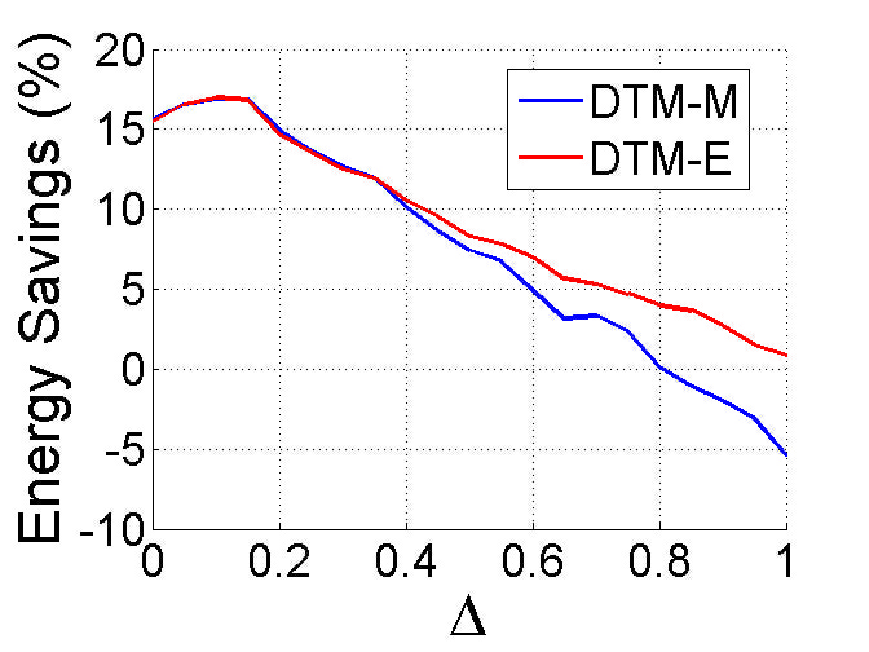
\includegraphics[width=\columnwidth]{./figures/flc_80_delta_energy}
%		\caption{Energy Experiment}
%		\label{fig:Flc80-delta-energy}
%	\end{subfigure}
%	\caption{Energy Savings for $F_{LC} = 80 MHz$ and utilization = 50\%.}
%	\label{fig:ins}
%\end{figure}	


\begin{figure*}[!tp]
	\centering
	\begin{subfigure}{.5\columnwidth}
		\centering
		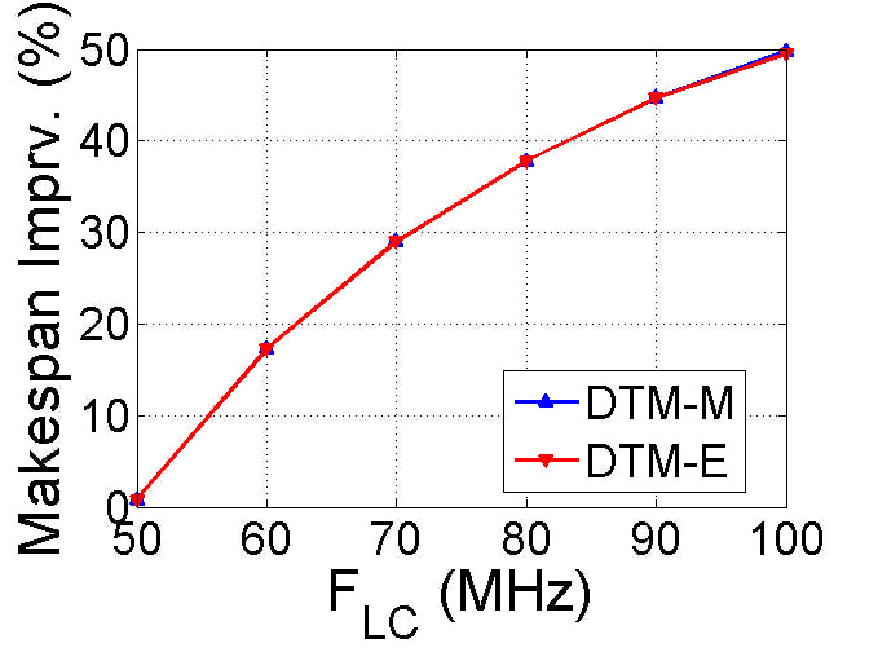
\includegraphics[width=\columnwidth]{./figures/flow_makespan}
		\caption{Makespan Improvement}
		\label{fig:flow_makespan}
	\end{subfigure}
	\begin{subfigure}{.5\columnwidth}
		\centering
		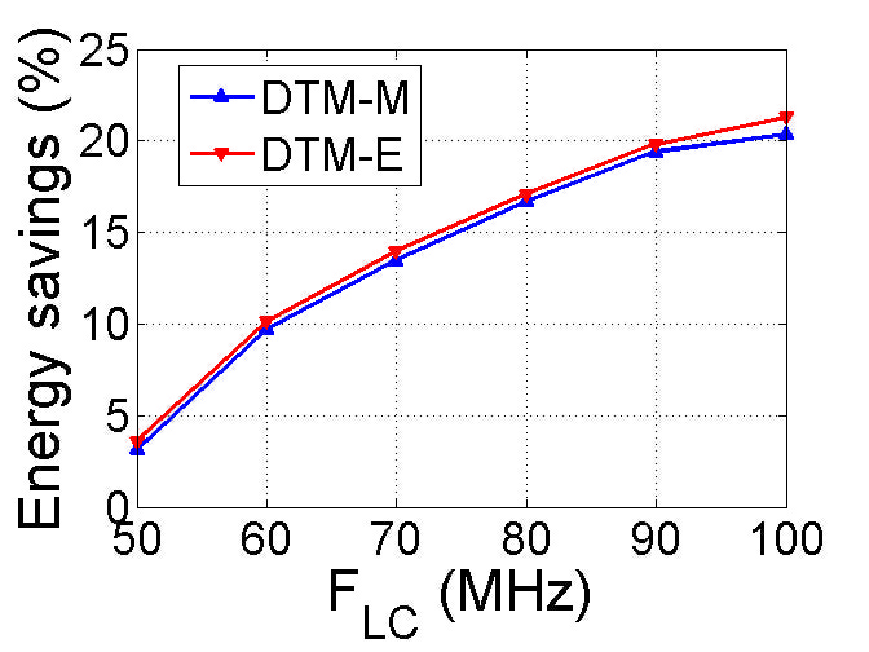
\includegraphics[width=\columnwidth]{./figures/flow_energy}
		\caption{Energy Savings}
		\label{fig:flow_energy}
	\end{subfigure}
	\begin{subfigure}{.5\columnwidth}
		\centering
		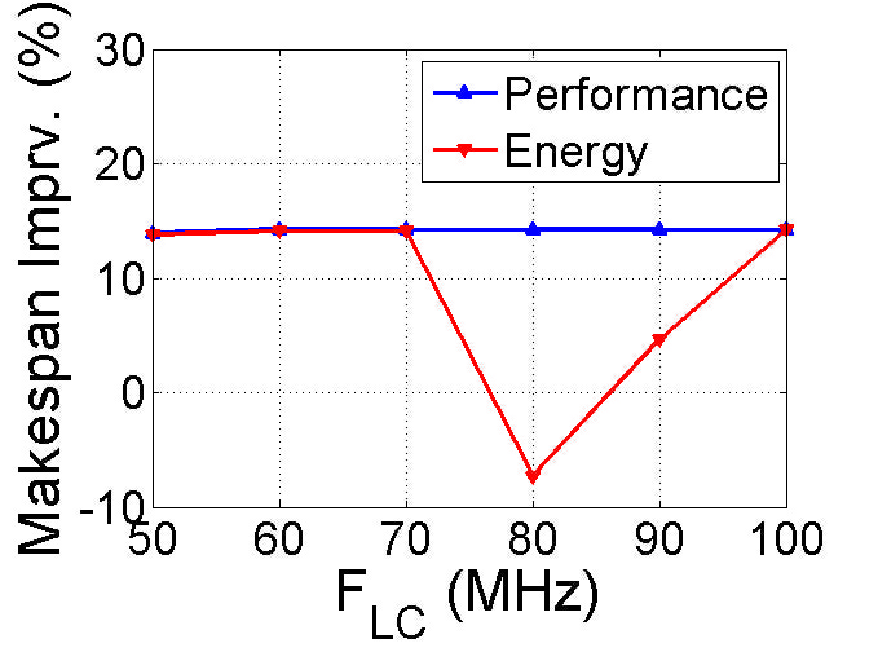
\includegraphics[width=\columnwidth]{./figures/openshoe_makespan}
		\caption{Makespan-INS}
		\label{fig:openshoe_makespan}
	\end{subfigure}
	\begin{subfigure}{.5\columnwidth}
		\centering
		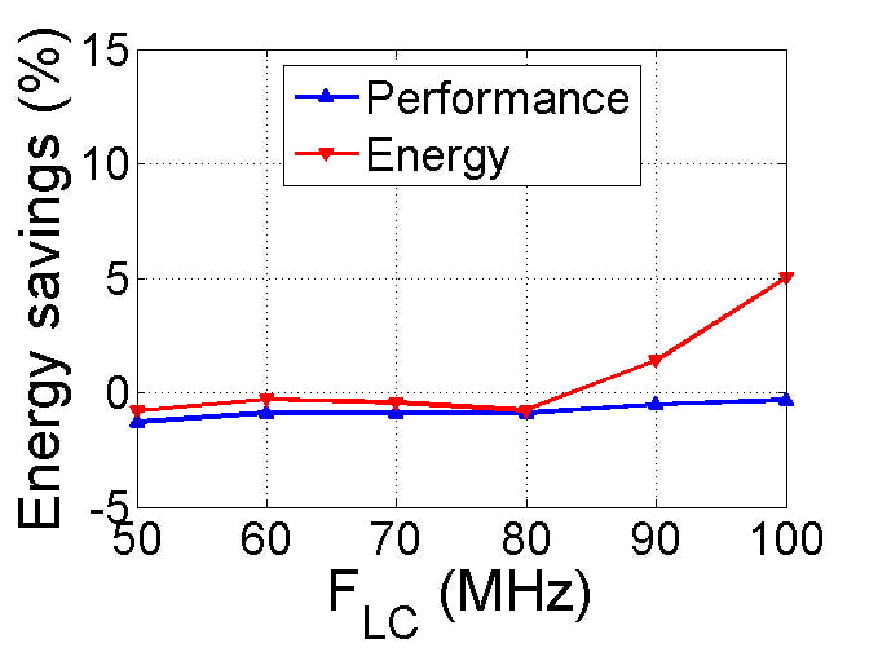
\includegraphics[width=\columnwidth]{./figures/openshoe_energy}
		\caption{Energy Savings-INS}
		\label{fig:openshoe_energy}
	\end{subfigure}
	\caption{Results for Pix4Flow and INS Benchmarks}
	\label{fig:Flc80-delta}
\end{figure*}

We first analyze the impact of single-core utilization on energy savings and makespan. In this set of experiments, we evaluate two values of $\Delta\in\{0.2, 0.5\}$. The results for this evaluation are presented in Figure~\ref{fig:Flc80-util}. In this case, the \% improvement in makespan remains constant as utilization is increased. Therefore, we plot the makespan improvement in the form of a bar graph in Figure~\ref{fig:Flc80-util-makespan}. %In the optimal case, the makespan is decreased by 44\% and the energy savings can reach up to 22\%. 
In general, the percentage improvement in energy consumption increases as the utilization increases. We have high energy savings when $\Delta = 0.2$, since it is close to $\Delta_\mathrm{opt}=\frac{100-80}{100+80}=0.11$. Furthermore, the two policies do not differ, as $\Delta \leq \Delta_\mathrm{diff}=0.37$. However, when $\Delta = 0.5$, the two policies differ and there is a tradeoff between performance and energy consumption. %Finally, it is important to mention that in both cases the Heavy-Light platform shows significant energy savings even for low utilization.\par

Now, we analyze the proposed schemes for different values of $\Delta$. Figure~\ref{fig:Flc80-delta} shows both theoretical results and experimental evaluation for utilization = 50\%. According to the plots, the optimal makespan improvement and energy savings are 44\% and 17\% respectively. Both $\Delta_\mathrm{opt}(\approx 0.11)$ and $\Delta_\mathrm{diff}(\approx 0.37)$ are in agreement with our theoretical findings. Though the amount of task-level parallelism, and consequently, the potential energy savings are highly application-dependent, we will show in the following section that different types of real-world applications can exhibit improvements in both energy and performance.
%Furthermore, as we illustrated in Figure~\ref{fig:delta-tasks}, a small number of tasks are required to coverage to the optimal value of $\Delta=\Delta_\mathrm{opt}$. Therefore, for majority of application scenarios, we will be operating close to $\Delta_\mathrm{opt}$, leading to high improvement in energy consumption and performance.

%By correlating Figures~\ref{fig:delta-tasks} and~\ref{fig:Flc80-delta} we can conclude that the combination of the Heavy-Light architecture and the MLPT heuristic can result into significant improvement both in performance and energy-consumption, even for a relatively low number of tasks. For example, for $F_{LC} = 80MHz$ and $n=5$ the makespan is reduced by 40\% and the energy consumption by 15\%. Even for $n=2$ the improvement in both metrics is non-negligible.\par

\noindent\textbf{Evaluation using Real-World Application:} In this evaluation, we demonstrate the impact of our policies on a real-world application. 
%We chose the Pix4Flow \cite{Pix4Flow} camera module, which serves as a reference for applications with high degree of task-level parallelism. This application corresponds to a workload with $\Delta = 0$ and utilization = 90\%. During these experiments, $F_{LC}$ is varied from $50MHz$ to $100MHz$ in steps of $10MHz$.
We consider two different embedded applications: 1) Pix4Flow \cite{Pix4Flow} camera module, 2) open-source Inertial Navigation System (INS)~\cite{INS}. Pix4Flow has high task level parallelism while INS has low task-level parallelism. Though the INS benchmark has dependencies between some tasks, we ignore them to determine the partitioning and respect them when executing the application. During these experiments, $F_{LC}$ is varied from $50MHz$ to $100MHz$ in steps of $10MHz$. %\textbf{(TODO: State $\Delta$s for these applications)} \par

As shown in Figures~\ref{fig:flow_makespan} and~\ref{fig:flow_energy}, in the case of the Pix4Flow benchmark, the differences between the two task allocation policies are very narrow. This is due to the high degree of task-level parallelism in this application. Interestingly, even in the pessimistic case of $F_{LC} = 50MHz$, both  policies offer approximately 4\% energy savings. Both makespan improvement and energy savings increase proportionally to $F_{LC}$ and can reach up to 50\% and 22\% respectively. %\par

%However, as shown in Figures~\ref{fig:openshoe_makespan} and~\ref{fig:openshoe_energy}, the two allocation policies show very different behavior in the case of the INS benchmark. The performance-oriented policy offers a constant makespan improvement of approximately 14\% and , due to the low task-level parallelism. 
%On the other hand, the allocation of tasks is not always the same in the case of the energy-efficient policy. As you can see in Figure~\ref{fig:openshoe_makespan}, for $F_{LC} = 80MHz$, the makespan starts increasing, until it reaches its maximum value again for $F_{LC} = 100MHz$. Moreover, the energy savings are also limited, reaching up to only 5\%. 

For the INS application, the two allocation policies show a very different behavior. This is shown in Figures~\ref{fig:openshoe_makespan} and~\ref{fig:openshoe_energy}. The difference is due to the low task-level parallelism present in the application. When $F_{LC} \geq 80MHz$, the two policies start differing. The energy-efficient policy shows a small improvement in energy consumption (up to 5\%). However, the improvement in energy comes at the cost of loss in performance; with makespan degradation of up to 8\% compared to single-core due to the LC executing the bigger task bin. The performance-oriented policy has a constant makespan improvement of approximately 14\% with a slight increase in energy consumption, since the larger task bin is always executed by the HC. %This result shows that our DTM algorithms can still be applied to dependent task-sets and obtain energy savings. %As mentioned earlier,  



%\begin{figure}[!btp]
%	\centering
%	\begin{subfigure}{.48\columnwidth}
%		\centering
%		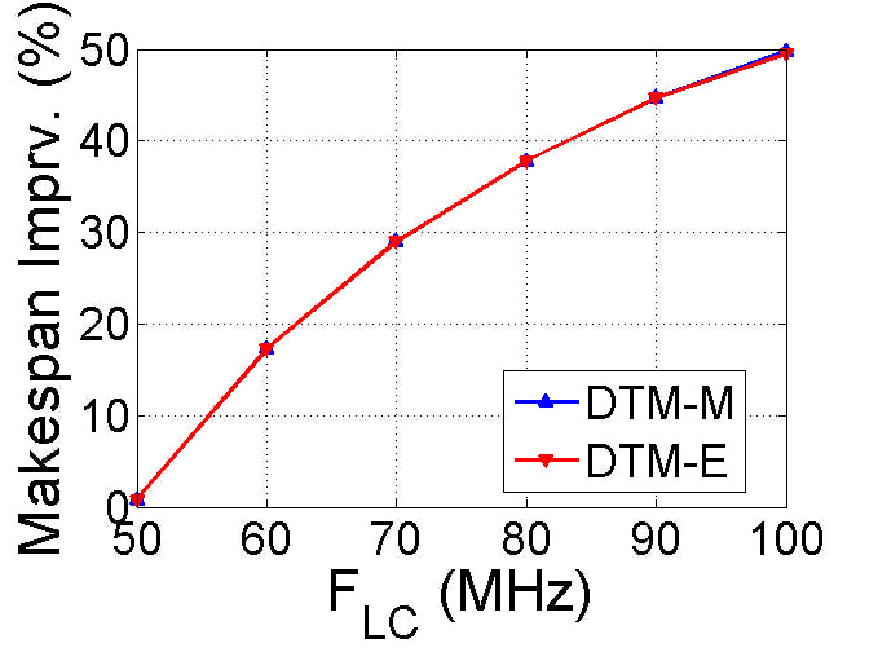
\includegraphics[width=\columnwidth]{./figures/flow_makespan}
%		\caption{Makespan Improvement}
%		\label{fig:flow_makespan}
%	\end{subfigure}
%	\begin{subfigure}{.48\columnwidth}
%		\centering
%		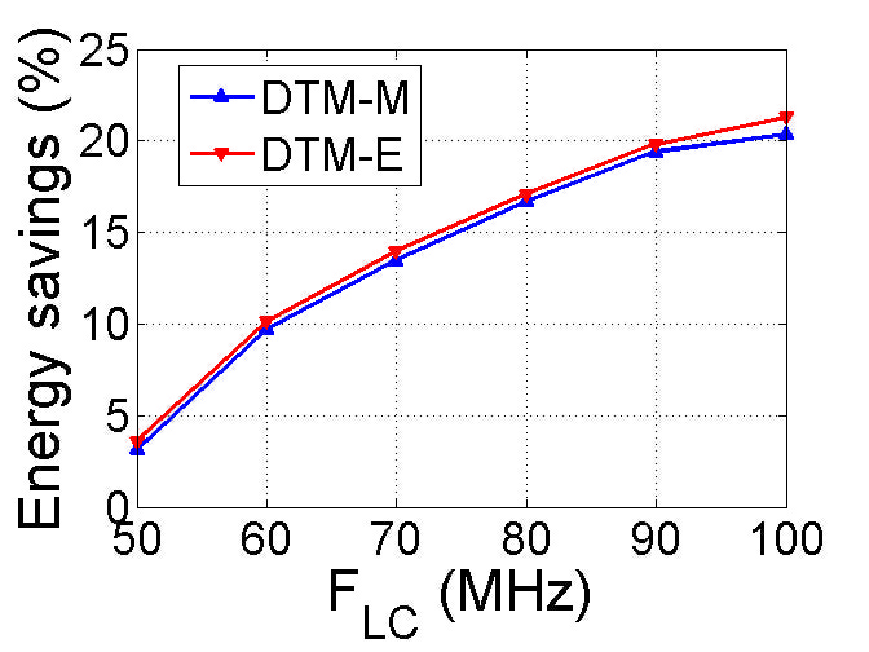
\includegraphics[width=\columnwidth]{./figures/flow_energy}
%		\caption{Energy Savings}
%		\label{fig:flow_energy}
%	\end{subfigure}
%	\caption{Results for Pix4Flow Benchmark}
%	\label{fig:flow}
%\end{figure}
%
%\begin{figure}[!btp]
%	\centering
%	\begin{subfigure}{.48\columnwidth}
%		\centering
%		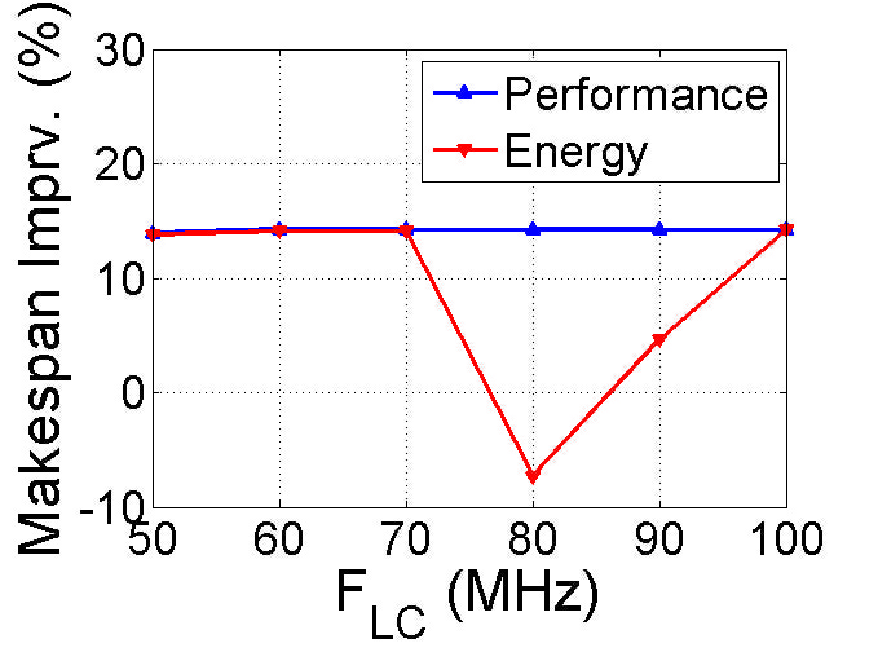
\includegraphics[width=\columnwidth]{./figures/openshoe_makespan}
%		\caption{Makespan-INS}
%		\label{fig:openshoe_makespan}
%	\end{subfigure}
%	\begin{subfigure}{.48\columnwidth}
%		\centering
%		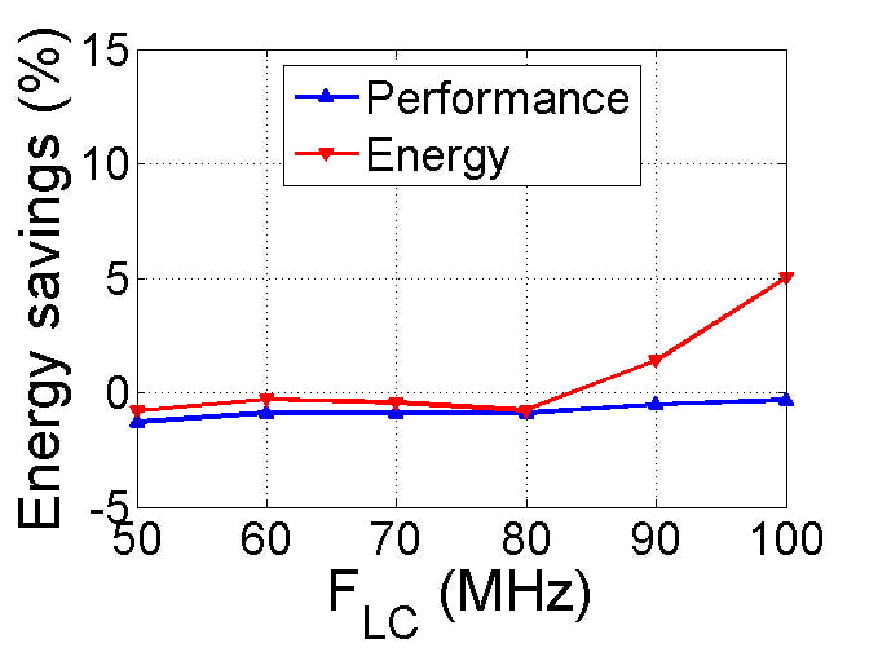
\includegraphics[width=\columnwidth]{./figures/openshoe_energy}
%		\caption{Energy Savings-INS}
%		\label{fig:openshoe_energy}
%	\end{subfigure}
%	\caption{Results for INS Benchmark}
%	\label{fig:ins}
%\end{figure}	



\section{Conclusion} \label{conclusion}
%%%%Conclusion%%%

In this work, we present a task allocation scheme which targets makespan and energy minimization, for the recently proposed Heavy-Light platform. We prove that only if the level is task-level parallelism is high enough, are the two objectives of minimizing makespan and minimizing energy equal. %Therefore, we do not have to tradeoff performance for energy efficiency. 
For scenarios where task level parallelism is low, we propose two Delta Threshold Mapping (DTM) policies which target performance (DTM-M) and energy (DTM-E). We theoretically prove the optimality of the proposed allocation policies and evaluate them on a hardware testbed. The results show an improvement of up to 50\% in makespan and up to 22\% in energy consumption; compared to a single-core platform.

%The current trends towards heterogeneous multi-core platforms and guardbands reductions, have opened new ways to address the energy consumption problem of MCUs. The recently proposed Heavy-Light architecture converges these trends with a platform capable of reducing the energy and makespan by only exploiting task-level parallelism. Furthermore, we have proven the optimality of our proposed task allocation scheme with respect to energy and makespan. For applications with enough available parallelism, our proposed policy can simultaneously minimize the application's energy and makespan. This optimality bound was proven mathematically and verified experimentally. Compared to state of the art policies on Heavy-Light architectures, our proposed policy holds valid for a wide range of operating frequencies, reaching up to 50\% in makespan reduction and up to 22\% in energy savings.

%Recent works have proposed hybrid architectures, consisting of one core designed to work reliably, independently on the environmental conditions (Heavy Core), and another designed to work under more relaxed conditions (Light Core). This work studies the impact of such an architecture on the performance and the energy consumption. We investigated different allocation scenarios and derived policies focusing both on reducing the makespan and maximizing the energy savings. Furthermore, we supported our proposals with mathematical proofs and validated the theoretical results by using emulation. Our results show substantial improvements, both in performance and energy consumption, reaching up to 50\% in makespan reduction and up to 24\% in energy savings, depending on the workload and platform characteristics.
%This work studies the impact of recently proposed hybrid architectures on the performance and energy consumption. We investigated different allocation scenarios and derived policies focusing both on reducing the makespan and maximizing the energy savings. Furthermore, we supported our proposals with mathematical proofs and validated the theoretical results by using emulation.
%\end{document}  % This is where a 'short' article might terminate

%ACKNOWLEDGMENTS are optional
%\section{Acknowledgments}
%This section is optional; it is a location for you
%to acknowledge grants, funding, editing assistance and
%what have you.  In the present case, for example, the
%authors would like to thank Gerald Murray of ACM for
%his help in codifying this \textit{Author's Guide}
%and the \textbf{.cls} and \textbf{.tex} files that it describes.

%
% The following two commands are all you need in the
% initial runs of your .tex file to
% produce the bibliography for the citations in your paper.


%\bibliographystyle{IEEETrans}
\bibliographystyle{etal}
\bibliography{refs}  

\end{document}
